\documentclass[8pt,a4paper,compress]{beamer}

\usepackage{/home/siyer/lib/slides}

\title{Type Checking}
\date{}

\begin{document}
\begin{frame}
\vfill
\titlepage
\end{frame}

\section{Introduction}
\begin{frame}[fragile]
\pause

Type checking (aka semantic analysis) is the final step in the analysis phase, and includes the following

\begin{itemize}
\pause
\item Determining the types of all names and expressions.
\pause
\item Insuring that all expressions are properly typed, for example that the operands of an operator have the proper types
\pause
\item A certain amount of storage analysis, for example determining the amount of storage that is required in the current stack frame to store a local variable (one word for \lstinline{int}s, two words for \lstinline{long}s); this information is used to allocate locations (at offsets from the base of the current stack frame) for parameters and local variables
\pause
\item A certain amount of AST tree rewriting, usually to make implicit constructs more explicit
\end{itemize}

\pause
\bigskip

Semantic analysis of \jmm programs involves all of the above
\end{frame}

\section{The \protect\jmm Types}
\begin{frame}[fragile]
\pause

A type in \jmm is either a primitive type or a reference type

\pause
\bigskip

\jmm primitive types
\begin{itemize}
\pause
\item \lstinline{int} - 32 bit two's complement integers
\pause
\item \lstinline{boolean} - taking the value \lstinline{true} or \lstinline{false}
\pause
\item \lstinline{char} - 16 bit Unicode (but many systems deal only with the lower 8 bits)
\end{itemize}

\pause
\bigskip

\jmm reference types
\begin{itemize}
\pause
\item arrays
\pause
\item objects of a type described by a class declaration
\pause
\item built-in objects \lstinline{java.lang.Object} and \lstinline{java.lang.String}
\end{itemize}

\pause
\bigskip

\jmm code may interact with classes from the Java library but it must be able to do so using only these types
\end{frame}

\begin{frame}[fragile]
\pause

How do we represent the types \lstinline{int}, \lstinline{int[]}, \lstinline{Factorial}, \lstinline{String[][]}?  

\pause
\bigskip

We want a simple, but extensible representation; we want no more complexity than is necessary for representing all of the types in \jmm and for representing any (Java) types that we may add in exercises

\pause
\bigskip

We want the ability to interact with the existing Java class libraries

\pause
\bigskip

Possible solutions
\begin{enumerate}
\pause
\item Java types are represented by objects of (Java) type \lstinline{java.lang.Class}; since \jmm is a subset of Java, why not use \lstinline{Class} objects to represent its types? 
\pause
\item Define an abstract class (or interface) \lstinline{Type}, and concrete sub-classes (or implementations) \lstinline{PrimitiveType}, \lstinline{ReferenceType}, and \lstinline{ArrayType}
\end{enumerate}
\end{frame}

\begin{frame}[fragile]
\pause

Our solution is to define our own class \lstinline{Type} for representing types, with a simple interface but also encapsulating the \lstinline{java.lang.Class} object that corresponds to the Java representation for that same type

\pause
\bigskip

Since the parser does not know anything about types, we define two placeholder type representations
\begin{enumerate}
\pause
\item \lstinline{TypeName} - for representing named types recognized by the parser like user-defined classes or imported classes until such time as they may be resolved to their proper \lstinline{Type} representation
\pause
\item \lstinline{ArrayTypeName} - for representing array types recognized by the parser like \lstinline{String[]}, until such time that they may resolved to their proper \lstinline{Type} representation
\end{enumerate}

\pause
\bigskip

During analysis, \lstinline{TypeName}s and \lstinline{ArrayTypeName}s are resolved to the \lstinline{Type}s that they represent

\pause
\bigskip

More specifically
\begin{itemize}
\pause
\item A \lstinline{TypeName} is resolved by looking it up in the current context, our symbol table representation, and the \lstinline{Type} found replaces the \lstinline{TypeName}, and finally, the \lstinline{Type}'s accessibility from the place the \lstinline{TypeName} is encountered is checked
\pause
\item Since an \lstinline{ArrayTypeName} has a base type, the base type is resolved to a \lstinline{Type}, whose \lstinline{Class} representation becomes the base type for representing the array type
\pause
\item A \lstinline{Type} resolves to itself
\end{itemize}
\end{frame}

\section{\protect\jmm Symbol Tables}
\begin{frame}[fragile]
\pause

A symbol table maps names to the things they name, for example, types, formal parameters and local variables; these mappings are established in a declaration and consulted each time a declared name is encountered

\pause
\bigskip

In the \jmm compiler, the symbol table is a tree of \lstinline{Context} objects, which spans the abstract syntax tree, with each \lstinline{Context} corresponding to a region of scope in the \jmm source program

\pause
\bigskip

For example, reconsider the simple \lstinline{Factorial} program.  In this version we mark two locations in the program using comments: \lstinline{position 1} and \lstinline{position 2}

\begin{lstlisting}[language=Java,style=focusin]
package pass;

import java.lang.System;

public class Factorial {
    public static int factorial(int n) {
        // position 1:
        if (n <= 0) {
            return 1;
        } else {
            return n * factorial(n - 1);
        }
    }

    public static void main(String[] args) {
        // position 2:
        int x = n;
        System.out.println(n + "! = " + factorial(x));
    }

    static int n = 5;
}
\end{lstlisting}
\end{frame}

\begin{frame}[fragile]
\pause

The symbol table for the \lstinline{Factorial} program, and its relationship to the AST, is illustrated in figure below

\begin{center}
\visible<2->{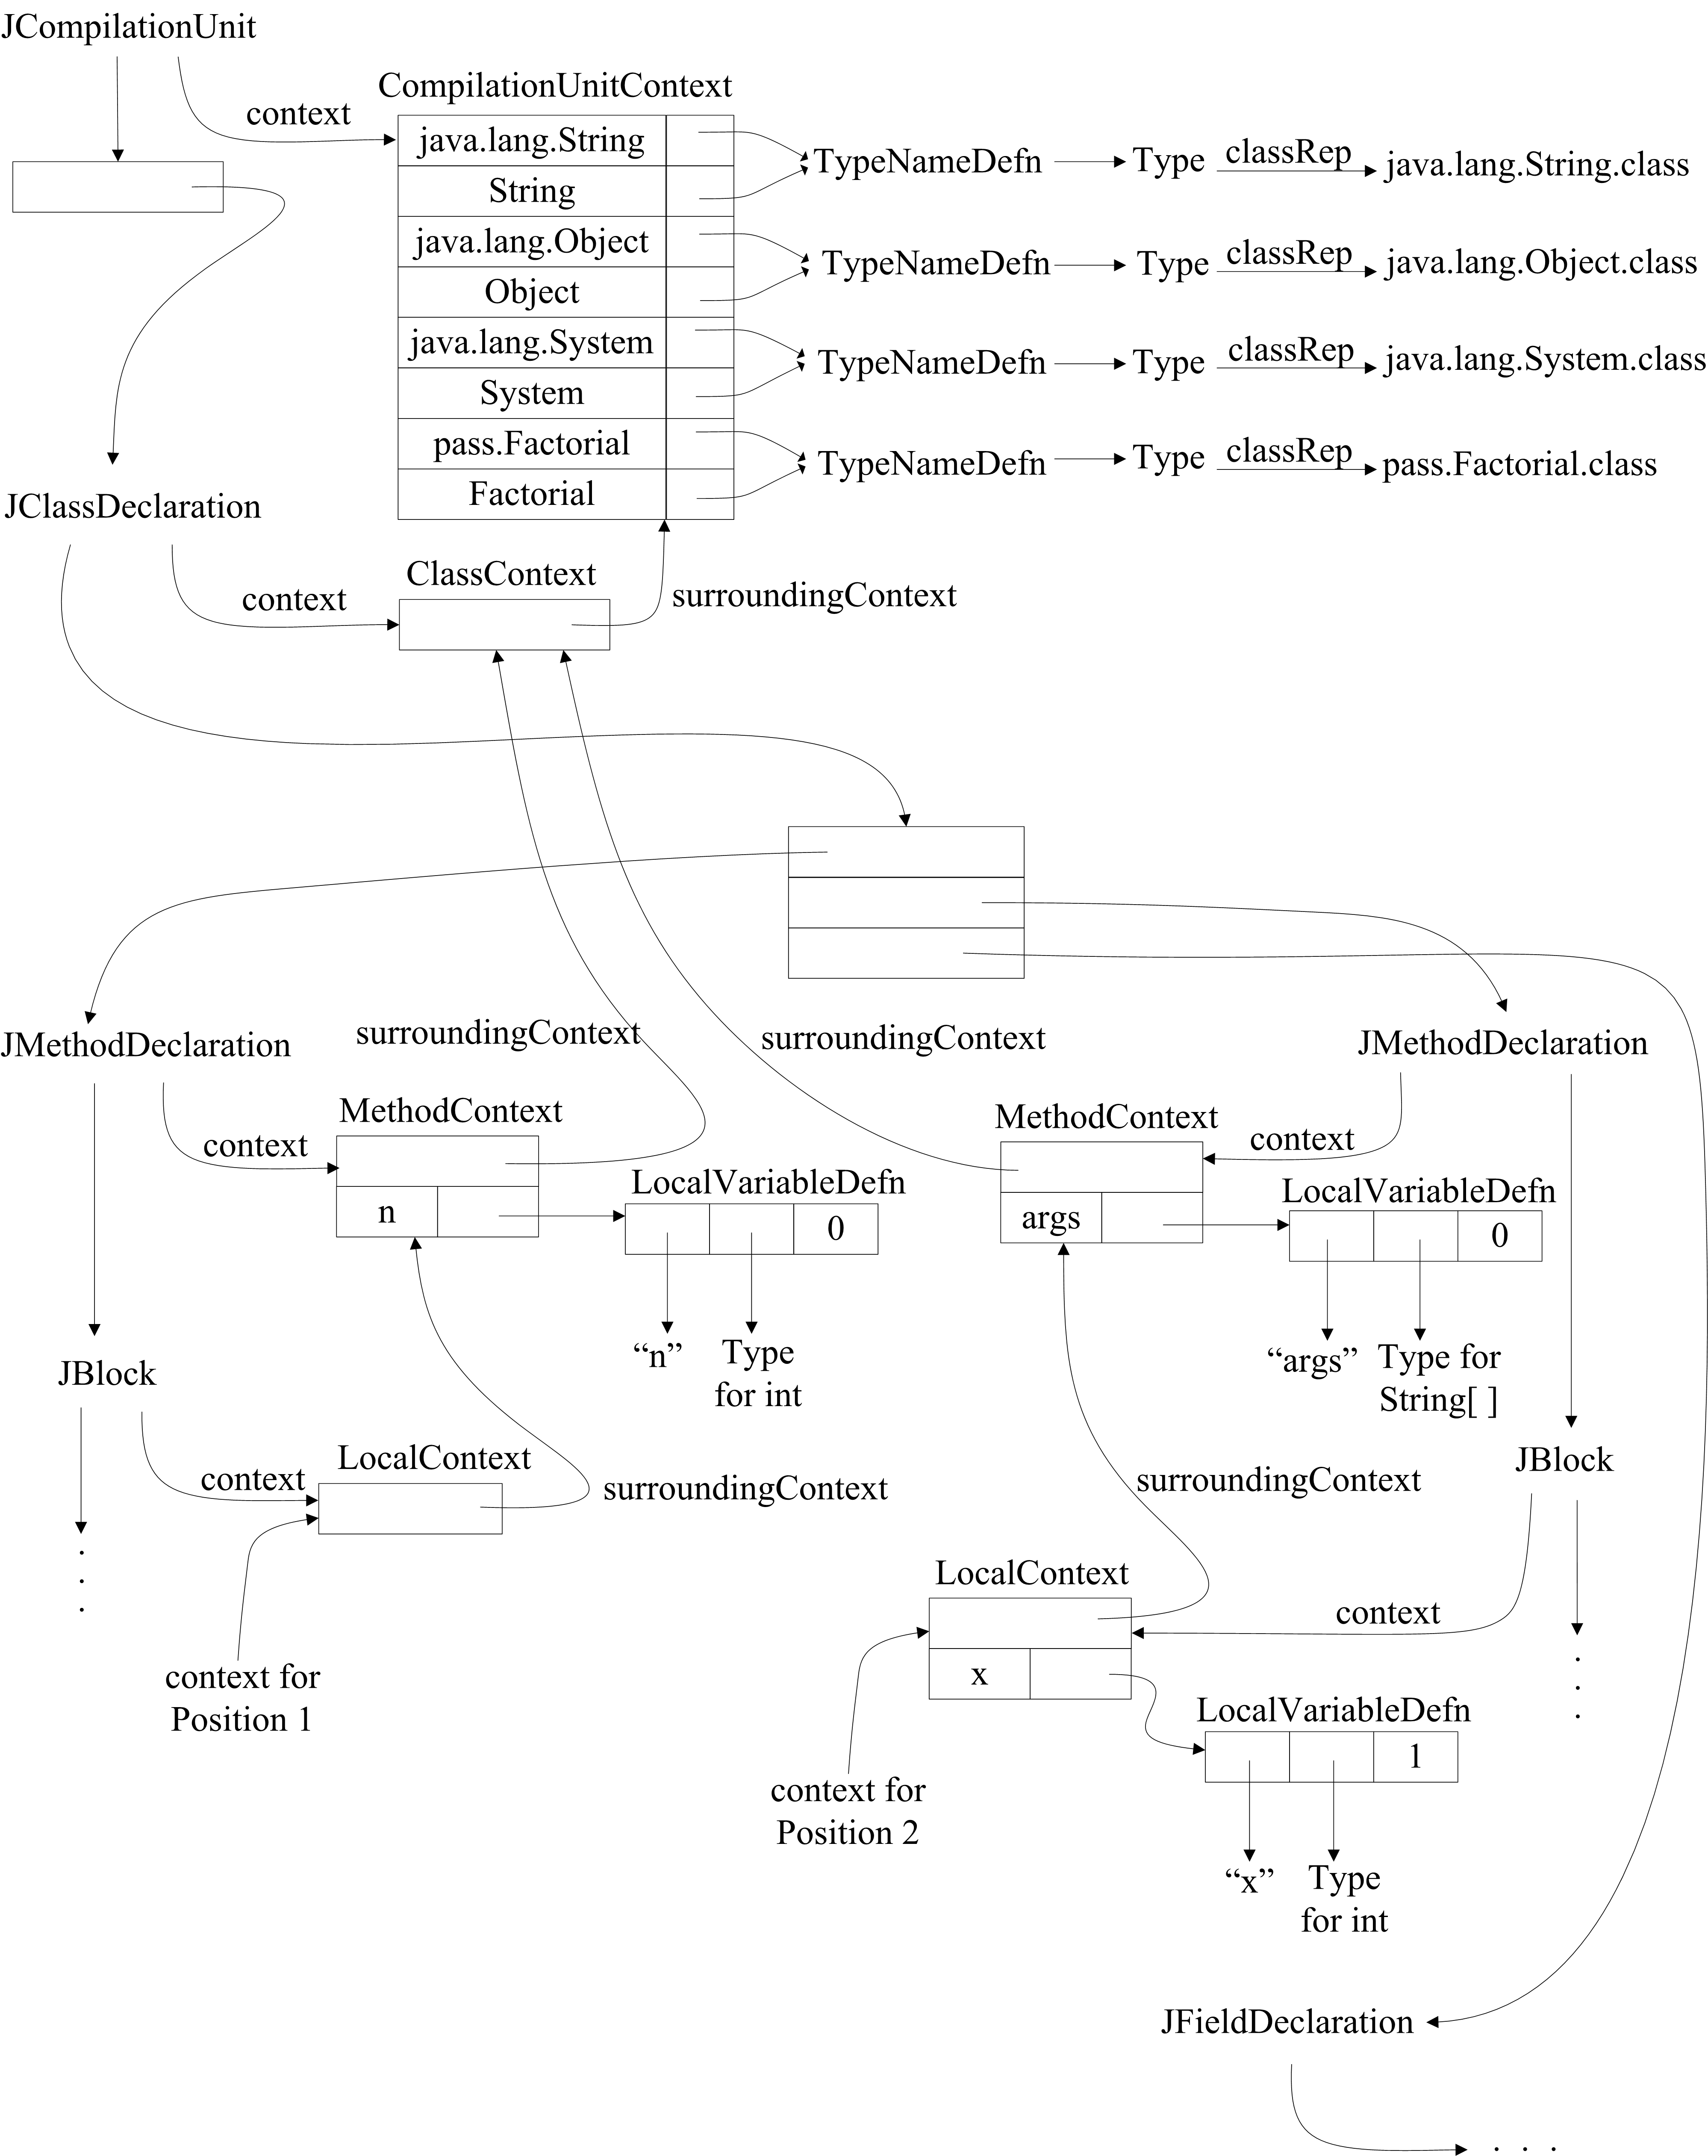
\includegraphics[scale=0.29]{{figures/figure04.01}.jpg}}
\end{center}
\end{frame}

\begin{frame}[fragile]
\pause

The symbol table takes the form of a tree that corresponds to the shape of the AST

\pause
\bigskip

A \lstinline{context}, ie, a node in this tree, captures the region of scope corresponding to the AST node that points to it

\pause
\bigskip

For example, in the above figure
\begin{enumerate}
\pause
\item The context pointer from the AST's \lstinline{JCompilationUnit} node points to the \lstinline{JCompilationUnitContext} that is at the root of the symbol table
\pause
\item The context pointer from the AST's \lstinline{JClassDeclaration} points to a \lstinline{ClassContext}
\pause
\item The context pointer from the AST's two \lstinline{JMethodDeclaration}s each point to a \lstinline{MethodContext}
\pause
\item The context pointer from the AST's two \lstinline{JBlock}s each point to a \lstinline{LocalContext}
\end{enumerate}

\pause
\bigskip

From any particular location in the program, looking back towards the root \lstinline{CompilationUnitContext}, the symbol table looks like a stack of contexts

\pause
\bigskip

Each \lstinline{surroundingContext} link back towards the \lstinline{CompilationUnitContext} points to the context representing the surrounding lexical scope
\end{frame}

\begin{frame}[fragile]
\pause

During analysis, when the compiler encounters a variable, it looks up that variable in the symbol table by name, beginning at the \lstinline{LocalContext} most recently created in the symbol table

\pause
\bigskip

Type names are looked up in the \lstinline{CompilationUnitContext}; to facilitate this, each context maintains three pointers to surrounding contexts, as illustrated in the following figure

\begin{center}
\visible<3->{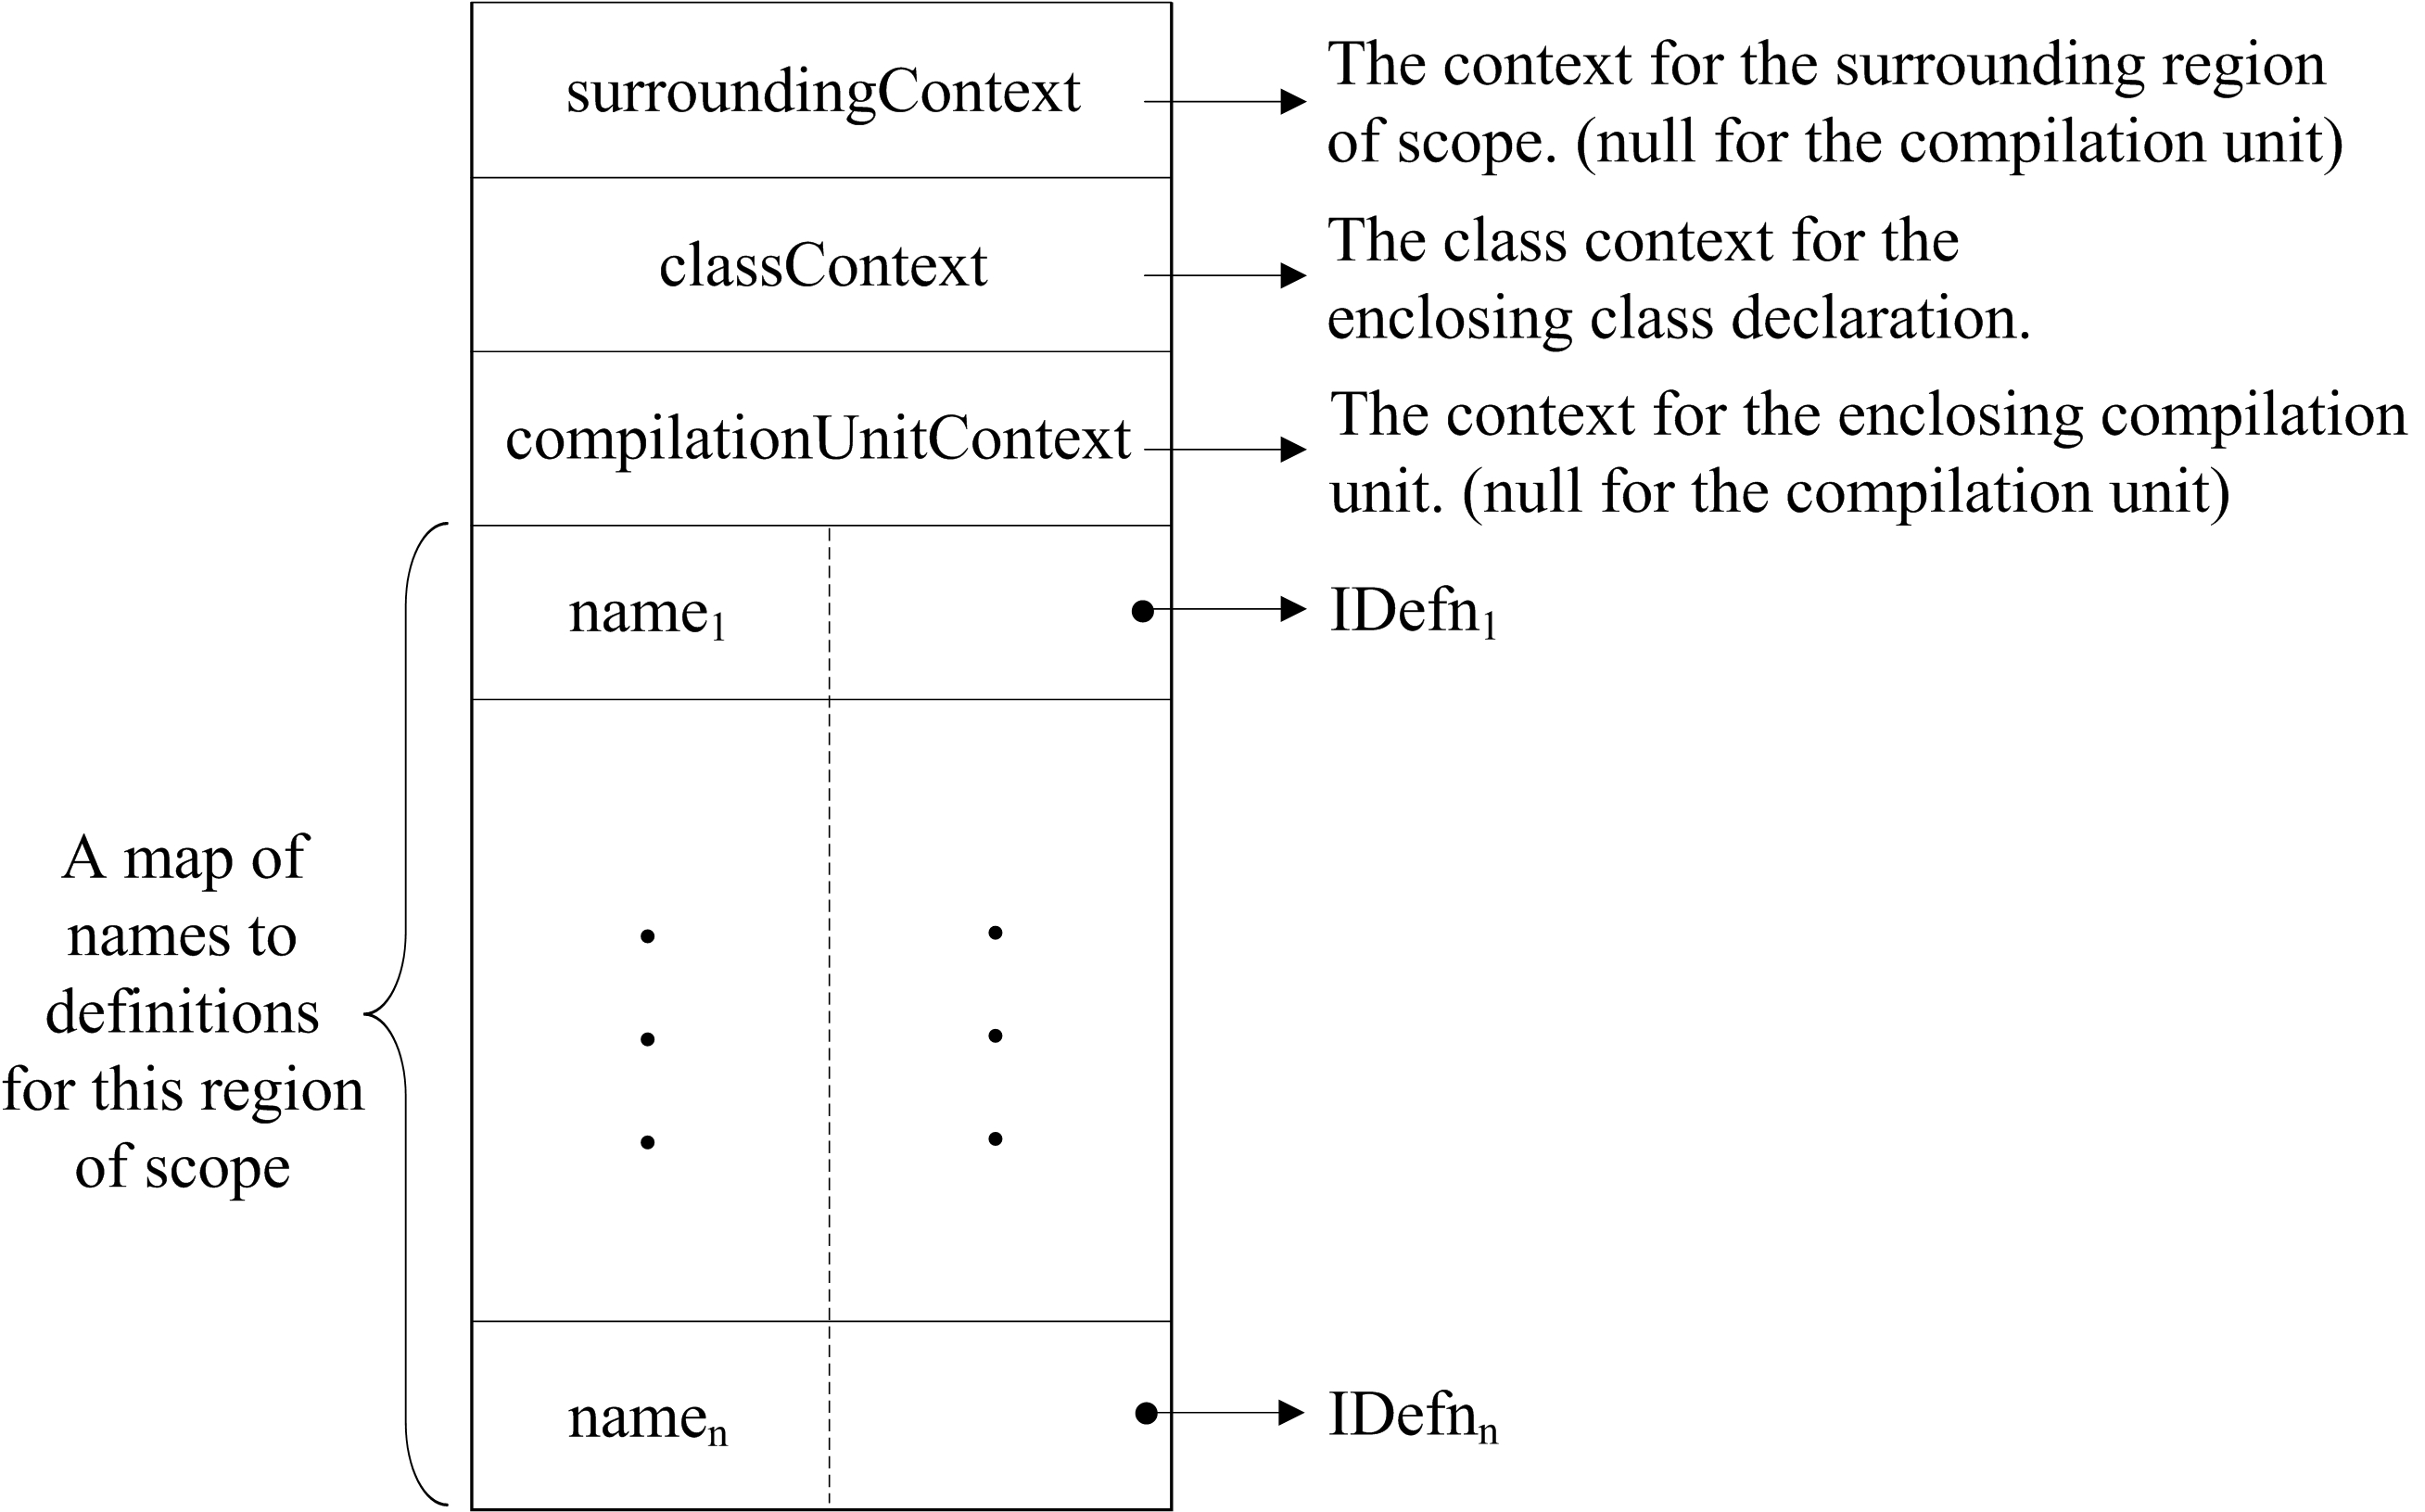
\includegraphics[scale=0.5]{{figures/figure04.02}.jpg}}
\end{center}
\end{frame}

\begin{frame}[fragile]
\pause

A \lstinline{CompilationUnitContext} represents the scope of the entire program and contains a mapping from names to types
\begin{itemize}
\pause
\item The implicitly declared types, \lstinline{java.lang.Object}, and \lstinline{java.lang.String}
\pause
\item Imported types
\pause
\item User-defined types, that is, types introduced in clss declarations
\end{itemize}

\pause
\bigskip

A \lstinline{ClassContext} represents the scope within a class declaration; in the \jmm symbol table, no names are declared here, but if we were to add nested type declarations to \jmm, they might be declared here

\pause
\bigskip

A \lstinline{MethodContext} represents the scope within a method declaration; a method's formal parameters are declared here

\pause
\bigskip

A \lstinline{LocalContext} represents the scope within a block, which includes the block defining the body to a method; local variables are declared here
\end{frame}

\begin{frame}[fragile]
\pause

Each kind of context derives from (extends) the class \lstinline{Context}, which supplies the mapping from names to definitions (\lstinline{IDefns})

\pause
\bigskip

The inheritance tree for contexts is illustrated in the following figure
\begin{center}
\visible<3->{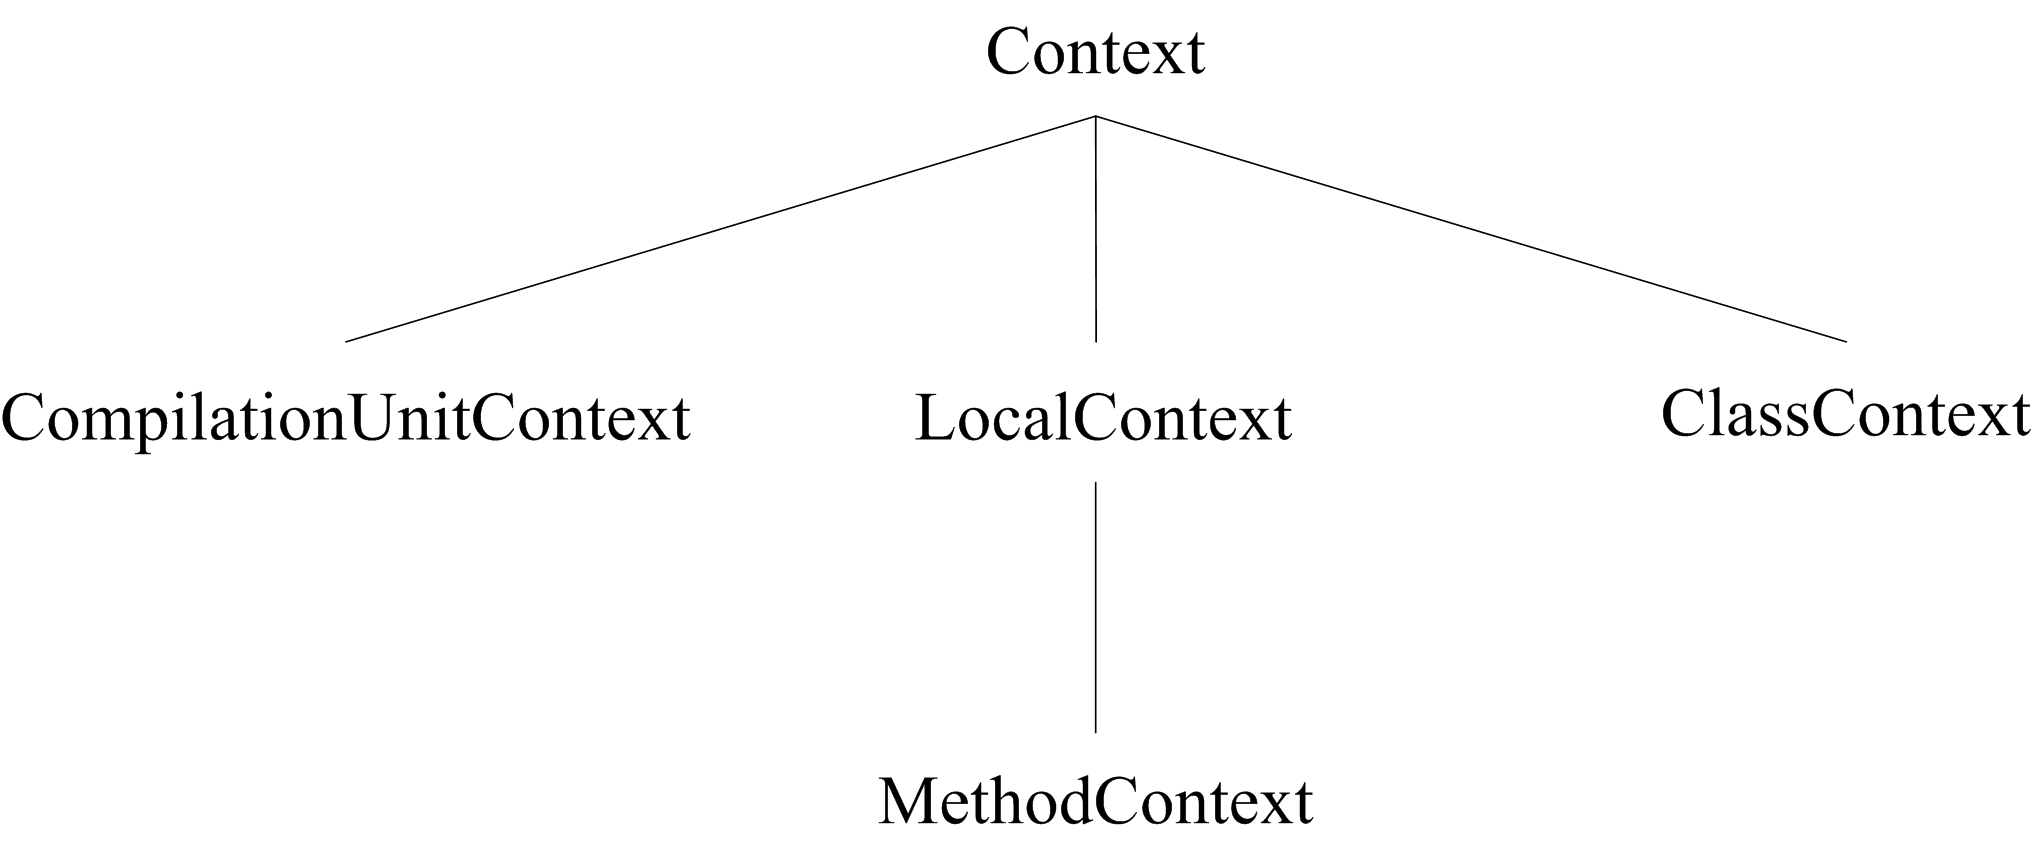
\includegraphics[scale=0.5]{{figures/figure04.03}.jpg}}
\end{center}

\pause
\bigskip

An \lstinline{IDefn} is the interface type for symbol table definitions, which has two implementations
\begin{enumerate}
\pause
\item A \lstinline{TypeNameDefn}, which defines a type name; an \lstinline{IDefn} of this sort encapsulates the \lstinline{Type} that it denotes
\pause
\item A \lstinline{LocalVariableDefn} defines a local variable and encapsulates the name, its \lstinline{Type} and an offset in the current run-time stack frame
\end{enumerate}
\end{frame}

\begin{frame}[fragile]
\pause

Class member (field and method in \jmm) names are not declared in a \lstinline{ClassContext}, but in the \lstinline{Type}s that they declare

\pause
\bigskip

We rely on the encapsulated \lstinline{Class} object to store the interface information, and we rely on Java reflection to query a type for information about its members

\pause
\bigskip

For example, \lstinline{Type} supports a method \lstinline{fieldFor()} which, when given a name returns a \lstinline{Field} with the given name that is defined for that type

\begin{lstlisting}[language=Java,style=focusin]
public Field fieldFor(String name) {
    Class<?> cls = classRep;
    while (cls != null) {
        java.lang.reflect.Field[] fields = cls.getDeclaredFields();
        for (java.lang.reflect.Field field:fields) {
            if (field.getName().equals(name)) {
                return new Field(field);
            }
        }
        cls = cls.getSuperclass();
    }
    return null;
}
\end{lstlisting}
\end{frame}

\section{Pre-analysis of \protect\jmm Programs}
\begin{frame}[fragile]
\pause

The semantic analysis of \jmm  programs requires two traversals of the AST because a class name or a member name may be referenced before it is declared in the source program

\pause
\bigskip

The traversals are accomplished by the method \lstinline{preAnalyze()} for the first traversal and the method \lstinline{analyze()} for the second, which invoke themselves at the child nodes for recursively descending the AST

\pause
\bigskip

The \lstinline{preAnalyze()} method must traverse down the AST only far enough for
\begin{itemize}
\pause
\item Declaring imported type names
\pause
\item Declaring user-defined class names
\pause
\item Declaring fields
\pause
\item Declaring methods (including their signatures - the types of their parameters)
\end{itemize}

\pause
\bigskip

Therefore, \lstinline{preAnalyze()}need be defined only in the following types of AST nodes
\begin{itemize}
\pause
\item \lstinline{JCompilationUnit}
\pause
\item \lstinline{JClassDeclaration}
\pause
\item \lstinline{JFieldDeclaration}
\pause
\item \lstinline{JMethodDeclaration}
\pause
\item \lstinline{JConstructorDeclaration}
\end{itemize}
\end{frame}

\begin{frame}[fragile]
\pause

For the \lstinline{JCompilationUnit} node at the top of the AST, \lstinline{preAnalyze()} does the following
\begin{enumerate}
\pause
\item It creates a \lstinline{CompilationUnitContext}
\pause
\item It declares the implicit \jmm types, \lstinline{java.lang.String} and \lstinline{java.lang.Object}
\pause
\item It declares any imported types
\pause
\item It declares the types defined by class declaration, ie, creates a \lstinline{Type} for each declared class, whose \lstinline{classRep} refers to a \lstinline{Class} object for an empty class; for example, in the pre-analysis phase of our \lstinline{Factorial} program above, the \lstinline{Type} for \lstinline{Factorial} would have a \lstinline{classRep}, the \lstinline{Class} object for the class
\begin{lstlisting}[language=Java,style=focusin]
class Factorial {}
\end{lstlisting}
\pause
\item Finally, \lstinline{preAnalyze()} invokes itself for each of the type declarations in the compilation unit
\end{enumerate}

\pause
\bigskip

Here is the code for \lstinline{preAnalyze()} in \lstinline{JCompilationUnit}
\begin{lstlisting}[language=Java,style=focusin]
public void preAnalyze() {
    context = new CompilationUnitContext();

    // Declare the two implicit types java.lang.Object and
    // java.lang.String
    context.addType(0, Type.OBJECT);
    context.addType(0, Type.STRING);
\end{lstlisting}
\end{frame}

\begin{frame}[fragile]
\pause

Here is the code for \lstinline{preAnalyze()} in \lstinline{JCompilationUnit}
\begin{lstlisting}[language=Java,style=focusin]

    // Declare any imported types
    for (TypeName imported: imports) {
        try {
            Class<?> classRep =
                Class.forName(imported.toString());
            context.addType(imported.line(),
                Type.typeFor(classRep));
        }
        catch (Exception e) {
            JAST.compilationUnit.reportSemanticError(
                imported.line(),
                "Unable to find %s", imported.toString());                      
        }
    }

    // Declare the locally declared type(s)
    CLEmitter.initializeByteClassLoader();
    for (JAST typeDeclaration: typeDeclarations) {
        ((JTypeDecl)
              typeDeclaration).declareThisType(context);
    }

    // Pre-analyze the locally declared type(s). Generate
    // (partial) Class instances, reflecting only the member
    // interface type information
    CLEmitter.initializeByteClassLoader();
    for (JAST typeDeclaration: typeDeclarations) {
        ((JTypeDecl)
          typeDeclaration).preAnalyze(context);
    }
}
\end{lstlisting}
\end{frame}

\begin{frame}[fragile]
\pause

In a class declaration, \lstinline{preAnalyze()} does the following
\begin{enumerate}
\pause
\item It firstly creates a new \lstinline{ClassContext}, whose \lstinline{surroundingContext} points to the \lstinline{CompilationUnitContext}
\pause
\item It resolves the class's super type
\pause
\item It creates a new \lstinline{CLEmitter} instance, which will eventually be converted to the \lstinline{Class} object for representing the declared class
\pause
\item It adds a class header, defining a name and any modifiers, to this \lstinline{CLEmitter} instance
\pause
\item It recursively invokes \lstinline{preAnalyze()} on each of the class's members, which causes field declarations, constructors and method declarations (but with empty bodies) to be added to the \lstinline{CLEmitter} instance
\pause
\item If there is no explicit constructor (having no arguments) in the set of members, it adds the implicit constructor to the \lstinline{CLEmitter} instance; for example, for the \lstinline{Factorial} program above, the following implicit constructor is added
\begin{lstlisting}[language=Java,style=focusin]
public Factorial() {
    super();
}
\end{lstlisting}
\pause
\item Finally, the \lstinline{CLEmitter} instance produces a \lstinline{Class} object, and that replaces the \lstinline{classRep} for the \lstinline{Type} of the declared class name in the (parent) \lstinline{ClassContext}
\end{enumerate}
\end{frame}

\begin{frame}[fragile]
\pause

Here is the code for \lstinline{preAnalyze()} in \lstinline{JClassDeclaration}
\begin{lstlisting}[language=Java,style=focusin]
public void preAnalyze(Context context) {
    // Construct a class context
    this.context = new ClassContext(this, context);

    // Resolve superclass
    superType = superType.resolve(this.context);

    // Creating a partial class in memory can result in a
    // java.lang.VerifyError if the semantics below are
    // violated, so we can't defer these checks to analyze()
    thisType.checkAccess(line, superType);
    if (superType.isFinal()) {
        JAST.compilationUnit.reportSemanticError(line,
            "Cannot extend a final type: %s",                                   
            superType.toString());
    }

    // Create the (partial) class
    CLEmitter partial = new CLEmitter();

    // Add the class header to the partial class
    String qualifiedName =
        JAST.compilationUnit.packageName() == "" ? name :
            JAST.compilationUnit.packageName() + "/" + name;
    partial.addClass(mods, qualifiedName, superType.jvmName(),
        null, false);
\end{lstlisting}
\end{frame}

\begin{frame}[fragile]
\pause

\begin{lstlisting}[language=Java,style=focusin]

    // Pre-analyze the members and add them to the partial class
    for (JMember member: classBlock) {
        member.preAnalyze(this.context, partial);
        if (member instanceof JConstructorDeclaration &&
             ((JConstructorDeclaration) member).
                 params.size() == 0) {
            hasExplicitConstructor = true;
        }
    }

    // Add the implicit empty constructor?
    if (!hasExplicitConstructor) {
        codegenPartialImplicitConstructor(partial);
    }

    // Get the Class rep for the (partial) class and make it the
    // representation for this type
    Type id = this.context.lookupType(name);
    if (id != null &&
         !JAST.compilationUnit.errorHasOccurred()) {
        id.setClassRep(partial.toClass());
    }
}
\end{lstlisting}
\end{frame}

\begin{frame}[fragile]
\pause

In a method declaration, \lstinline{preAnalyze()} does the following
\begin{enumerate}
\pause
\item It resolves the types of the formal parameters
\pause
\item It resolves the return type
\pause
\item It checks proper use of the \lstinline{abstract} modifier
\pause
\item It computes the method descriptor
\pause
\item It generates (partial) code for the method
\end{enumerate}

\pause
\bigskip

Here is the code for \lstinline{preAnalyze()} in \lstinline{JMethodDeclaration}
\begin{lstlisting}[language=Java,style=focusin]
public void preAnalyze(Context context, CLEmitter partial) {
    // Resolve types of the formal parameters
    for (JFormalParameter param: params) {
        param.setType(param.type().resolve(context));
    }

    // Resolve return type
    returnType = returnType.resolve(context);
    
\end{lstlisting}
\end{frame}

\begin{frame}[fragile]
\pause

\begin{lstlisting}[language=Java,style=focusin]
    // Check proper local use of abstract
    if (isAbstract && body != null) {
        JAST.compilationUnit.reportSemanticError(line(),
            "abstract method cannot have a body");
    }
    else if (body == null && ! isAbstract) {
        JAST.compilationUnit.reportSemanticError(line(),
            "Method with null body must be abstract");
    }
    else if (isAbstract && isPrivate ) {
        JAST.compilationUnit.reportSemanticError(line(),
            "private method cannot be declared abstract");
    }
    else if (isAbstract && isStatic ) {
        JAST.compilationUnit.reportSemanticError(line(),
            "static method cannot be declared abstract");
    }

    // Compute descriptor
    descriptor = "(";
    for (JFormalParameter param: params) {
        descriptor += param.type().toDescriptor();
    }
    descriptor += ")" + returnType.toDescriptor();

    // Generate the method with an empty body (for now)
    partialCodegen(context, partial);
}
\end{lstlisting}
\end{frame}

\begin{frame}[fragile]
\pause

The code for \lstinline{partialCodegen()} is as follows
\begin{lstlisting}[language=Java,style=focusin]
public void partialCodegen(Context context, CLEmitter partial) {
    // Generate a method with an empty body; need a return to
    // make the class verifier happy.
    partial.addMethod(mods, name, descriptor, null, false);

    // Add implicit RETURN
    if (returnType == Type.VOID) {
	partial.addNoArgInstruction(RETURN);
    }
    else if (returnType == Type.INT ||
              returnType == Type.BOOLEAN ||
              returnType == Type.CHAR) {
        partial.addNoArgInstruction(ICONST_0);
        partial.addNoArgInstruction(IRETURN);
    }
    else {
        // A reference type.
        partial.addNoArgInstruction(ACONST_NULL);
        partial.addNoArgInstruction(ARETURN);
    }
}
\end{lstlisting}
\end{frame}

\begin{frame}[fragile]
\pause

Pre-analysis for a \lstinline{JFieldDeclaration} is similar to that for a \lstinline{JMethodDeclaration}, and does the following
\begin{enumerate}
\pause
\item Enforces the rule that fields may not be declared \lstinline{abstract}
\pause
\item Resolves the field's declared type
\pause
\item Generates the JVM code for the field declaration, via the \lstinline{CLEmitter} created for the enclosing class declaration
\end{enumerate}

\pause
\bigskip

The code itself is rather simple
\begin{lstlisting}[language=Java,style=focusin]
public void preAnalyze(Context context, CLEmitter partial) {
    // Fields may not be declared abstract.
    if (mods.contains("abstract")) {
        JAST.compilationUnit.reportSemanticError(line(),
            "Field cannot be declared abstract");
    }

    for (JVariableDeclarator decl: decls) {
        // Add field to (partial) class
        decl.setType(decl.type().resolve( context));
        partial.addField(mods, decl.name(),
            decl.type().toDescriptor(), false);
    }
}
\end{lstlisting}
\end{frame}

\begin{frame}[fragile]
\pause

The following figure illustrates how much of the symbol table is constructed for our \lstinline{Factorial} program once pre-analysis is complete

\begin{center}
\visible<2->{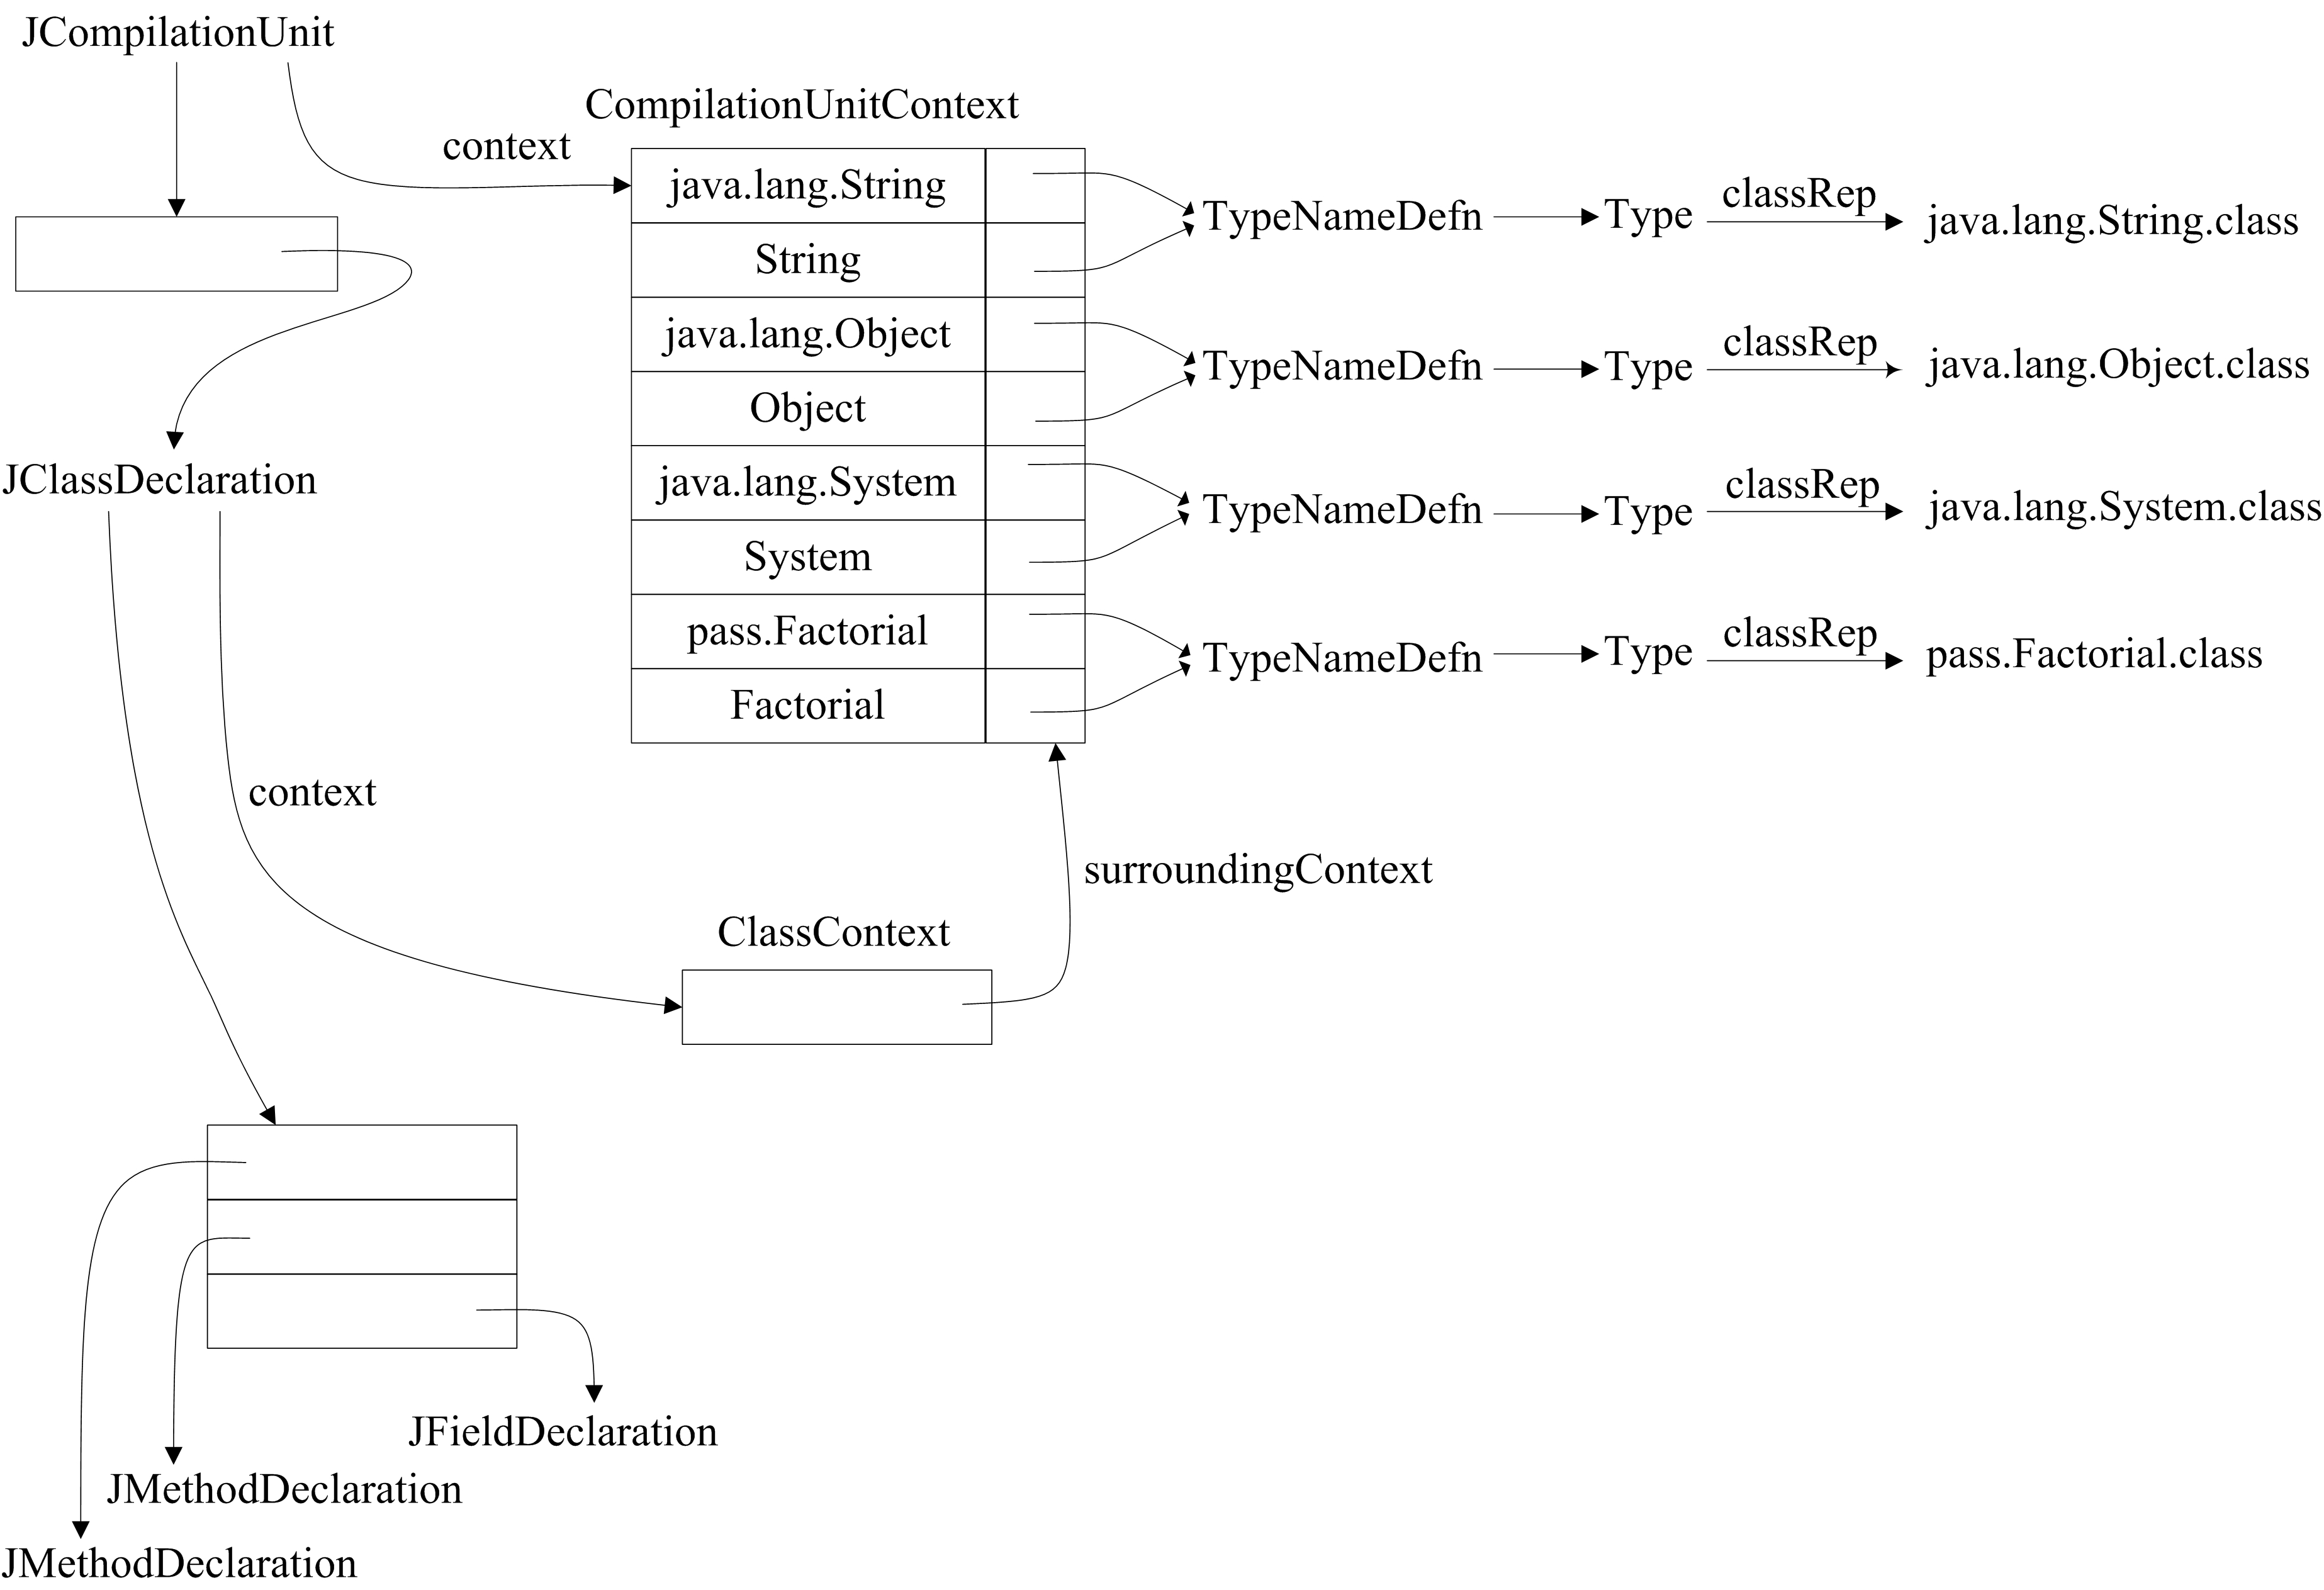
\includegraphics[scale=0.5]{{figures/figure04.04}.jpg}}
\end{center}
\end{frame}

\section{Analysis of \protect\jmm Programs}
\begin{frame}[fragile]
\pause

The analysis phase, ie, the \lstinline{analyze()} method, recursively descends throughout the AST all the way to its leaves
\begin{itemize}
\pause
\item Re-writing field and local variable initializations as assignments
\pause
\item Declaring both formal parameters and local variables
\pause
\item Allocating locations in the stack frame for the formal parameters and local variables
\pause
\item Computing the types of expressions and enforcing the language type rules
\pause
\item Reclassifying ambiguous names
\pause
\item Doing a limited amount of tree surgery
\end{itemize}

\pause
\bigskip

At the top of the AST, \lstinline{analyze()} simply recursively descends into each of the  type (class) declarations, delegating analysis to one class declaration at a time
\begin{lstlisting}[language=Java,style=focusin]
public JAST analyze(Context context) {
    for (JAST typeDeclaration : typeDeclarations) {
        typeDeclaration.analyze(this.context);
    }
    return this;
}
\end{lstlisting}
\end{frame}

\begin{frame}[fragile]
\pause

In \lstinline{JFieldDeclaration}, \lstinline{analyze()} rewrites the field initializer as an explicit assignment statement, analyzes that and then stores it in the \lstinline{JFieldDeclaration}'s initializations list
\begin{lstlisting}[language=Java,style=focusin]
public JFieldDeclaration analyze(Context context) {
    for (JVariableDeclarator decl : decls) {
        // All initializations must be turned into assignment
        // statements and analyzed
        if (decl.initializer() != null) {
            JAssignOp assignOp = new JAssignOp(decl.line(), 
                                     new JVariable(decl.line(), 
                                         decl.name()), decl.initializer());
            assignOp.isStatementExpression = true;
            initializations.add(new JStatementExpression(decl.line(), 
                                assignOp).analyze(context));
        }
    }
    return this;
}
\end{lstlisting}

\pause
\bigskip

In \lstinline{JClassDeclaration}, \lstinline{analyze()} separates the assignment statements into two lists: one for the static fields and one for the instance fields
\begin{lstlisting}[language=Java,style=focusin]
// Copy declared fields for purposes of initialization.
for (JMember member : classBlock) {
    if (member instanceof JFieldDeclaration) {
        JFieldDeclaration fieldDecl = (JFieldDeclaration) member;
        if (fieldDecl.mods().contains("static")) {
            staticFieldInitializations.add(fieldDecl);
        } else {
            instanceFieldInitializations.add(fieldDecl);
        }
    }
}
\end{lstlisting}
\end{frame}

\begin{frame}[fragile]
\pause

The following figure shows how the static field declaration (\lstinline{static int n = 5;}) in the \lstinline{Factorial} program is rewritten
\begin{center}
\visible<2->{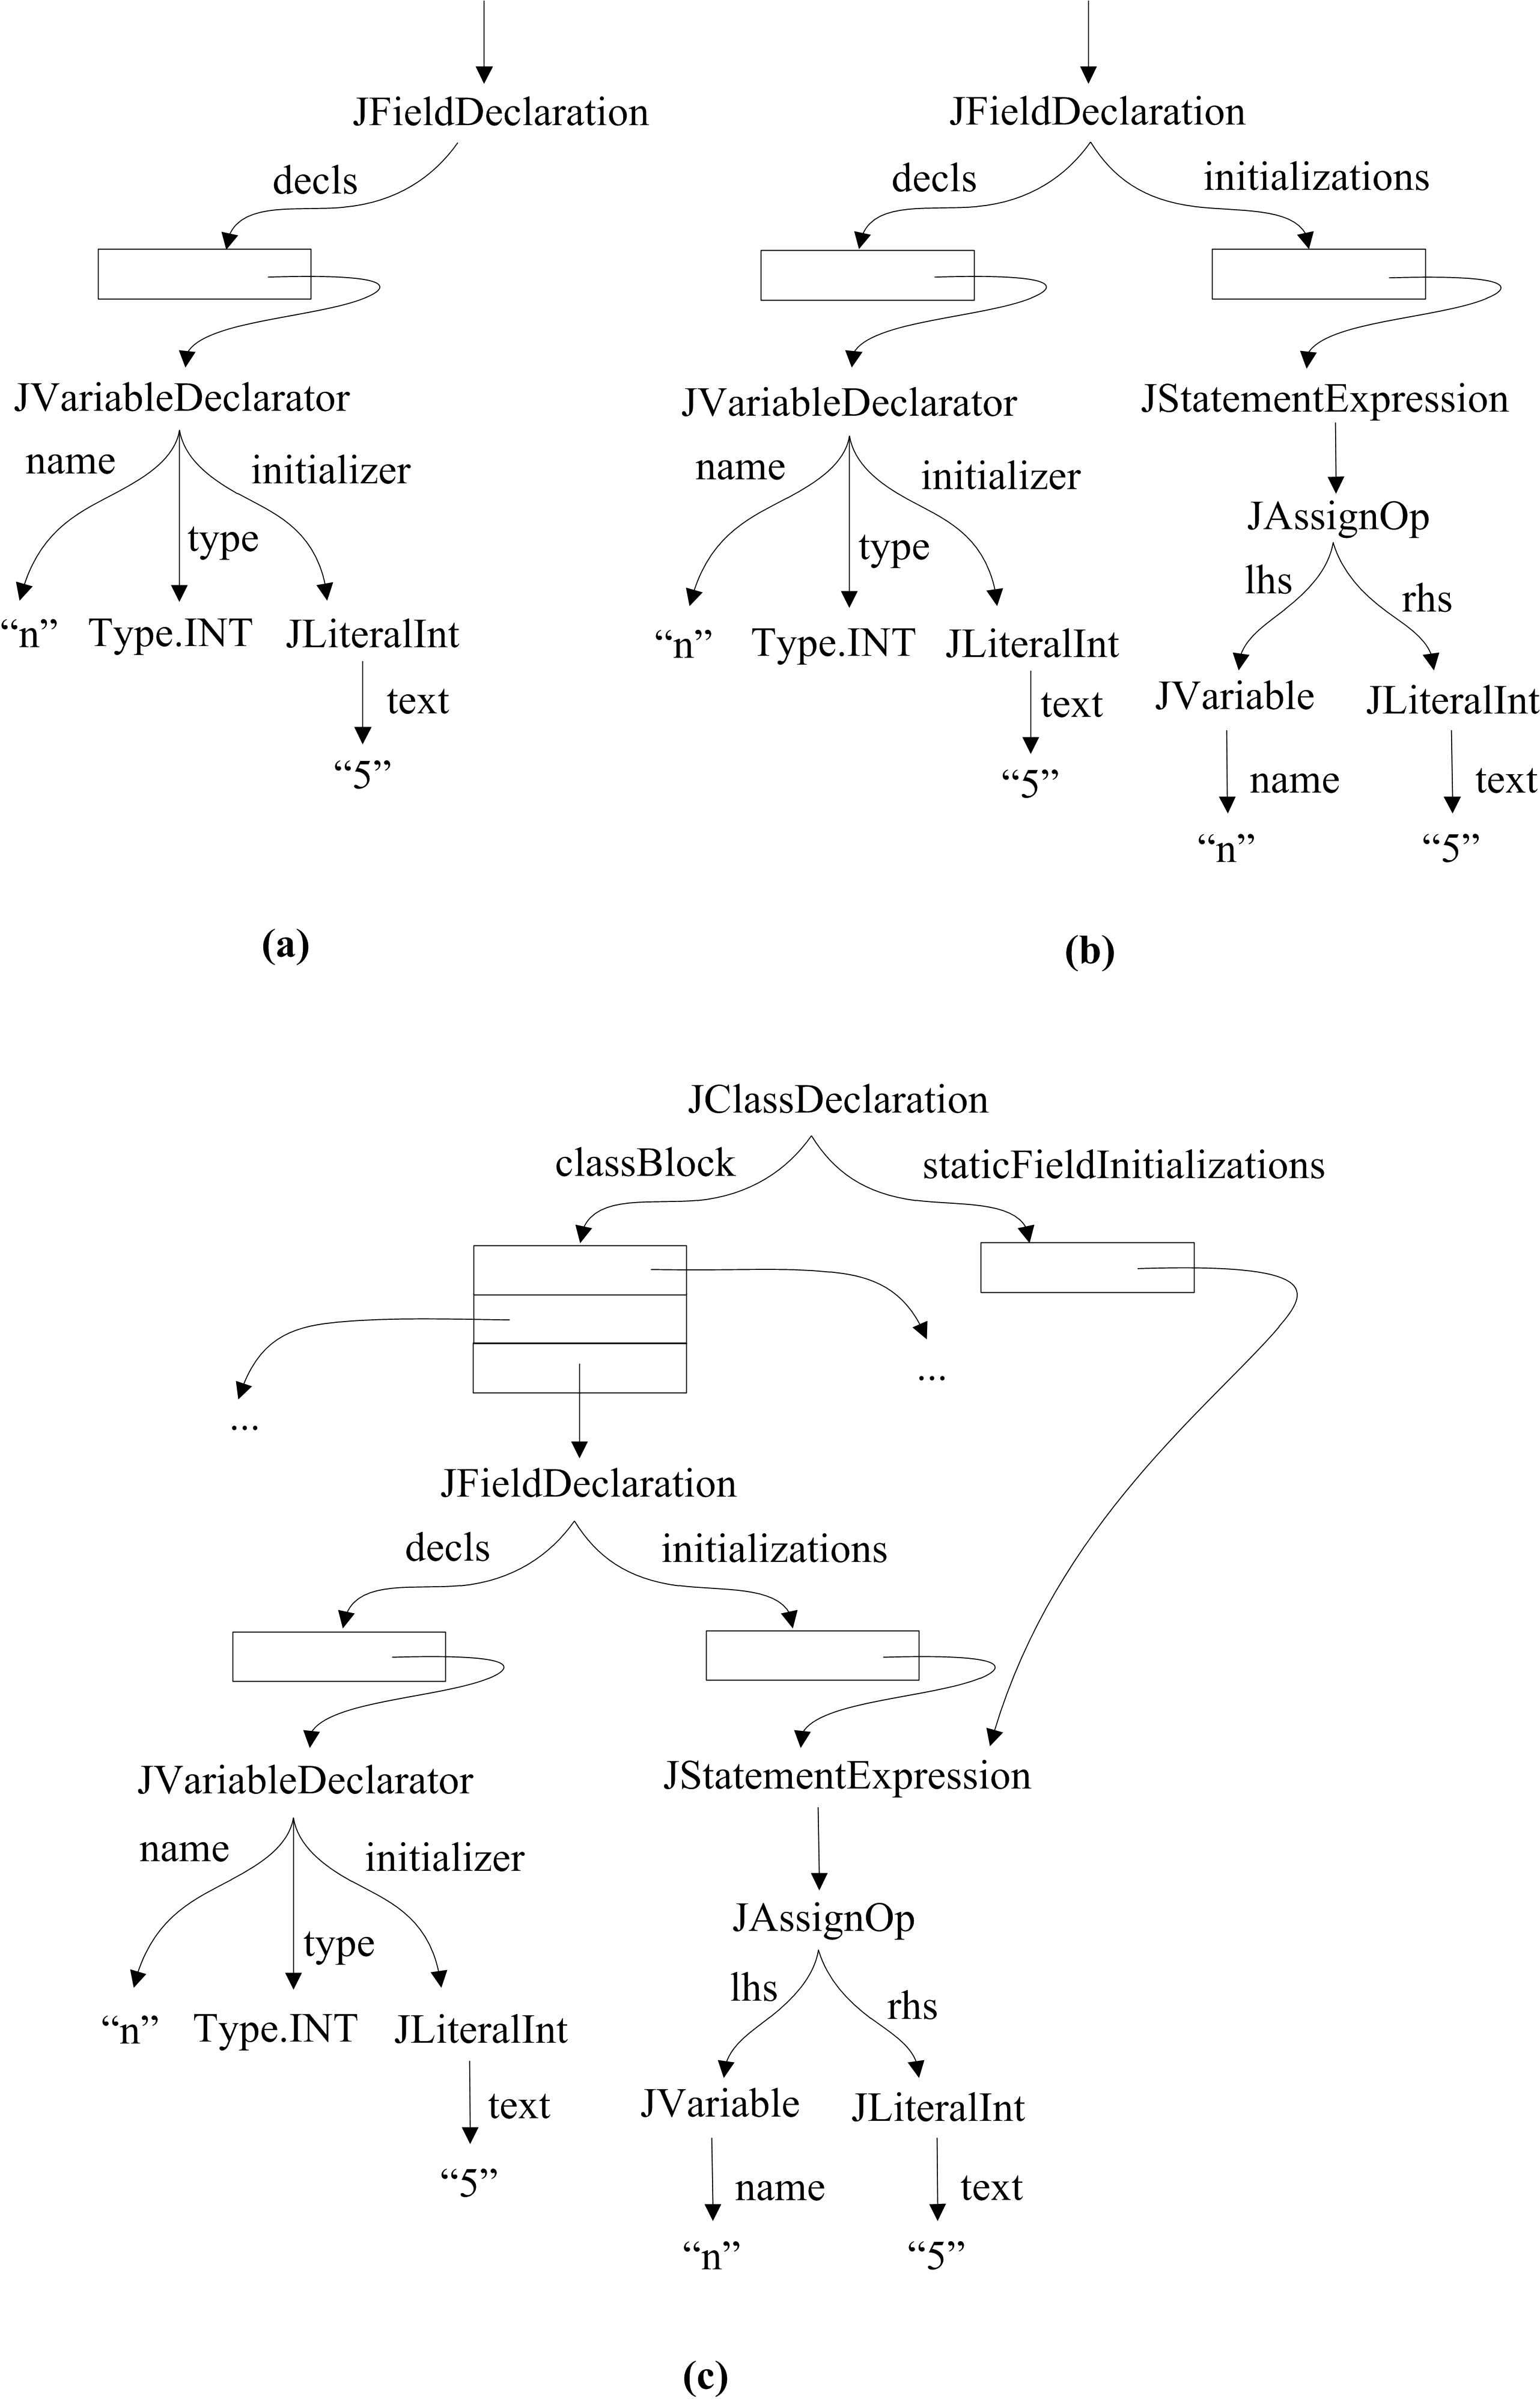
\includegraphics[scale=0.35]{{figures/figure04.05}.jpg}}
\end{center}
\end{frame}

\begin{frame}[fragile]
\pause

Both formal parameters and local variables are declared in the symbol table and allocated locations within a method invocation's run-time stack frame

\pause
\bigskip

For example, consider the following class declaration
\begin{lstlisting}[language=Java,style=focusin]
public class Locals {
    public int foo(int t, String u) {
        int v = u.length();
        {
            int w = v + 5, x = w + 7;
            v = w + x;
        }
        {
            int y = 3;
            int z = v + y;
            t = t + y + z;
        }
        return t + v;
    }
}
\end{lstlisting}
\end{frame}

\begin{frame}[fragile]
\pause

The stack frame allocated for an invocation of \lstinline{foo()} at run time by the JVM is shown below
\begin{center}
\visible<2->{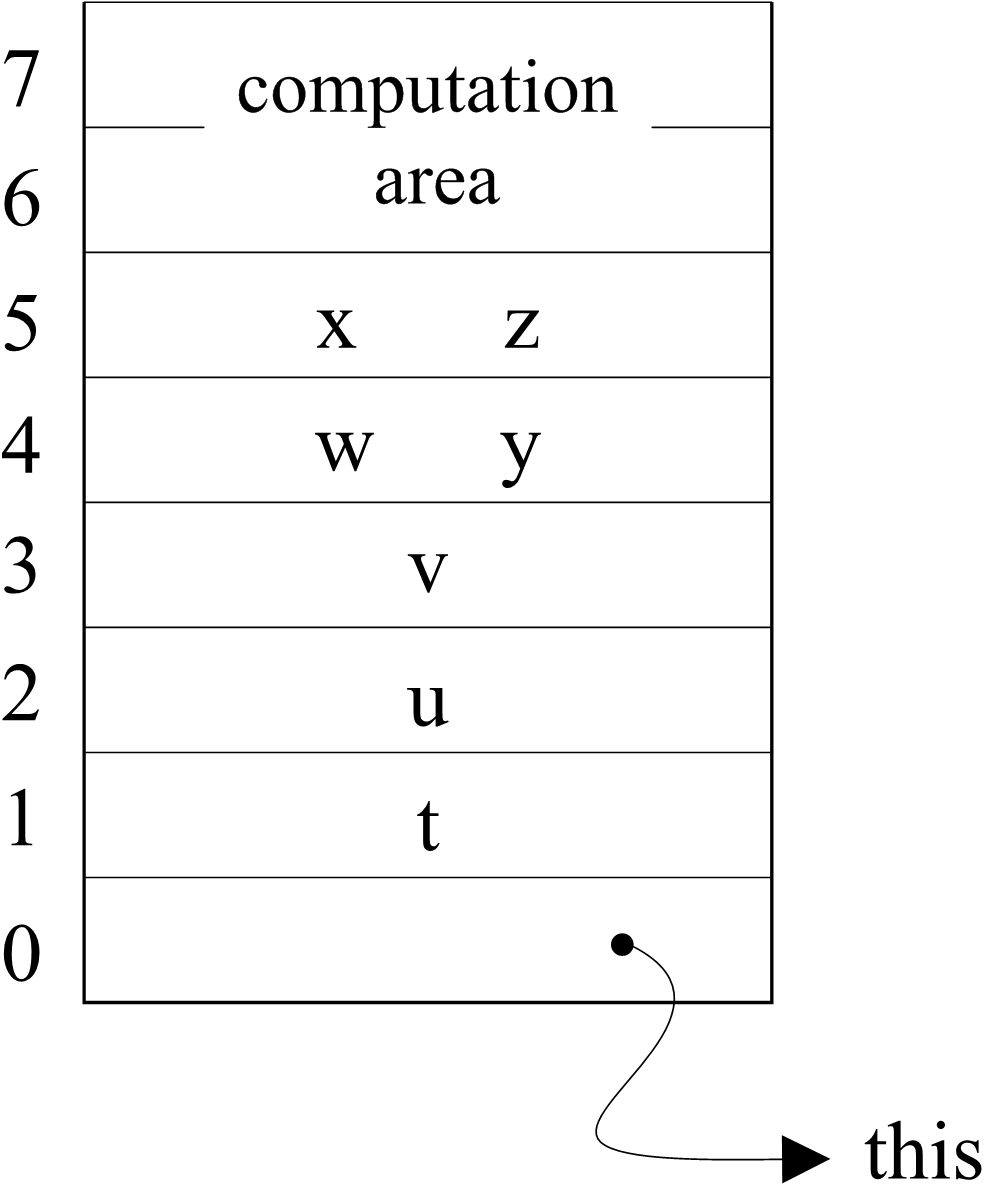
\includegraphics[scale=0.5]{{figures/figure04.06}.jpg}}
\end{center}

\pause
\bigskip

The code for analyzing a \lstinline{JMethodDeclaration} performs four steps
\begin{enumerate}
\pause
\item It creates a new \lstinline{MethodContext}, whose \lstinline{surroundingContext} points back to the previous \lstinline{ClassContext}
\pause
\item The first stack frame offset is 0; but if this is an instance method then offset 0 must be allocated to \lstinline{this}, and the \lstinline{nextOffset} is incremented to 1
\pause
\item The formal parameters are declared as local variables and allocated consecutive offsets in the stack frame
\pause
\item It analyzes the method's body
\end{enumerate}
\end{frame}

\begin{frame}[fragile]
\pause

\begin{lstlisting}[language=Java,style=focusin]
public JAST analyze(Context context) {
    this.context = new MethodContext(context, returnType);

    if (!isStatic) {
        // Offset 0 is used to addr "this".
        this.context.nextOffset();
    }

    // Declare the parameters
    for (JFormalParameter param : params) {
        this.context.addEntry(param.line(), param.name(),
                new LocalVariableDefn(param.type(), this.context
                        .nextOffset(), null));
    }

    if (body != null) {
        body = body.analyze(this.context);
    }
    return this;
}
\end{lstlisting}
\end{frame}

\begin{frame}[fragile]
\pause

The code for analyzing a \lstinline{JBlock} performs two steps
\begin{enumerate}
\pause
\item It creates a new \lstinline{LocalContext}, whose \lstinline{surroundingContext} points back to the previous \lstinline{MethodContext} (or \lstinline{LocalContext} in the case of nested blocks); its \lstinline{nextOffset} value is copied from the previous context
\pause
\item It analyzes each of the body's statements; any \lstinline{JVariableDeclaration}s declare their variables in the \lstinline{LocalContext} created in step 1; any nested \lstinline{JBlock} simply invokes this two-step process recursively, creating yet another \lstinline{LocalContext} for the nested block
\end{enumerate}

\pause
\bigskip

\begin{lstlisting}[language=Java,style=focusin]
public JBlock analyze(Context context) {
    // { ... } defines a new level of scope.
    this.context = new LocalContext(context);

    for (int i = 0; i < statements.size(); i++) {
        statements.set(i, (JStatement) statements.get(i).analyze(
                this.context));
    }
    return this;
}
\end{lstlisting}
\end{frame}

\begin{frame}[fragile]
\pause

The stages of the symbol table in analyzing \lstinline{Locals.foo()}
\begin{center}
\visible<2->{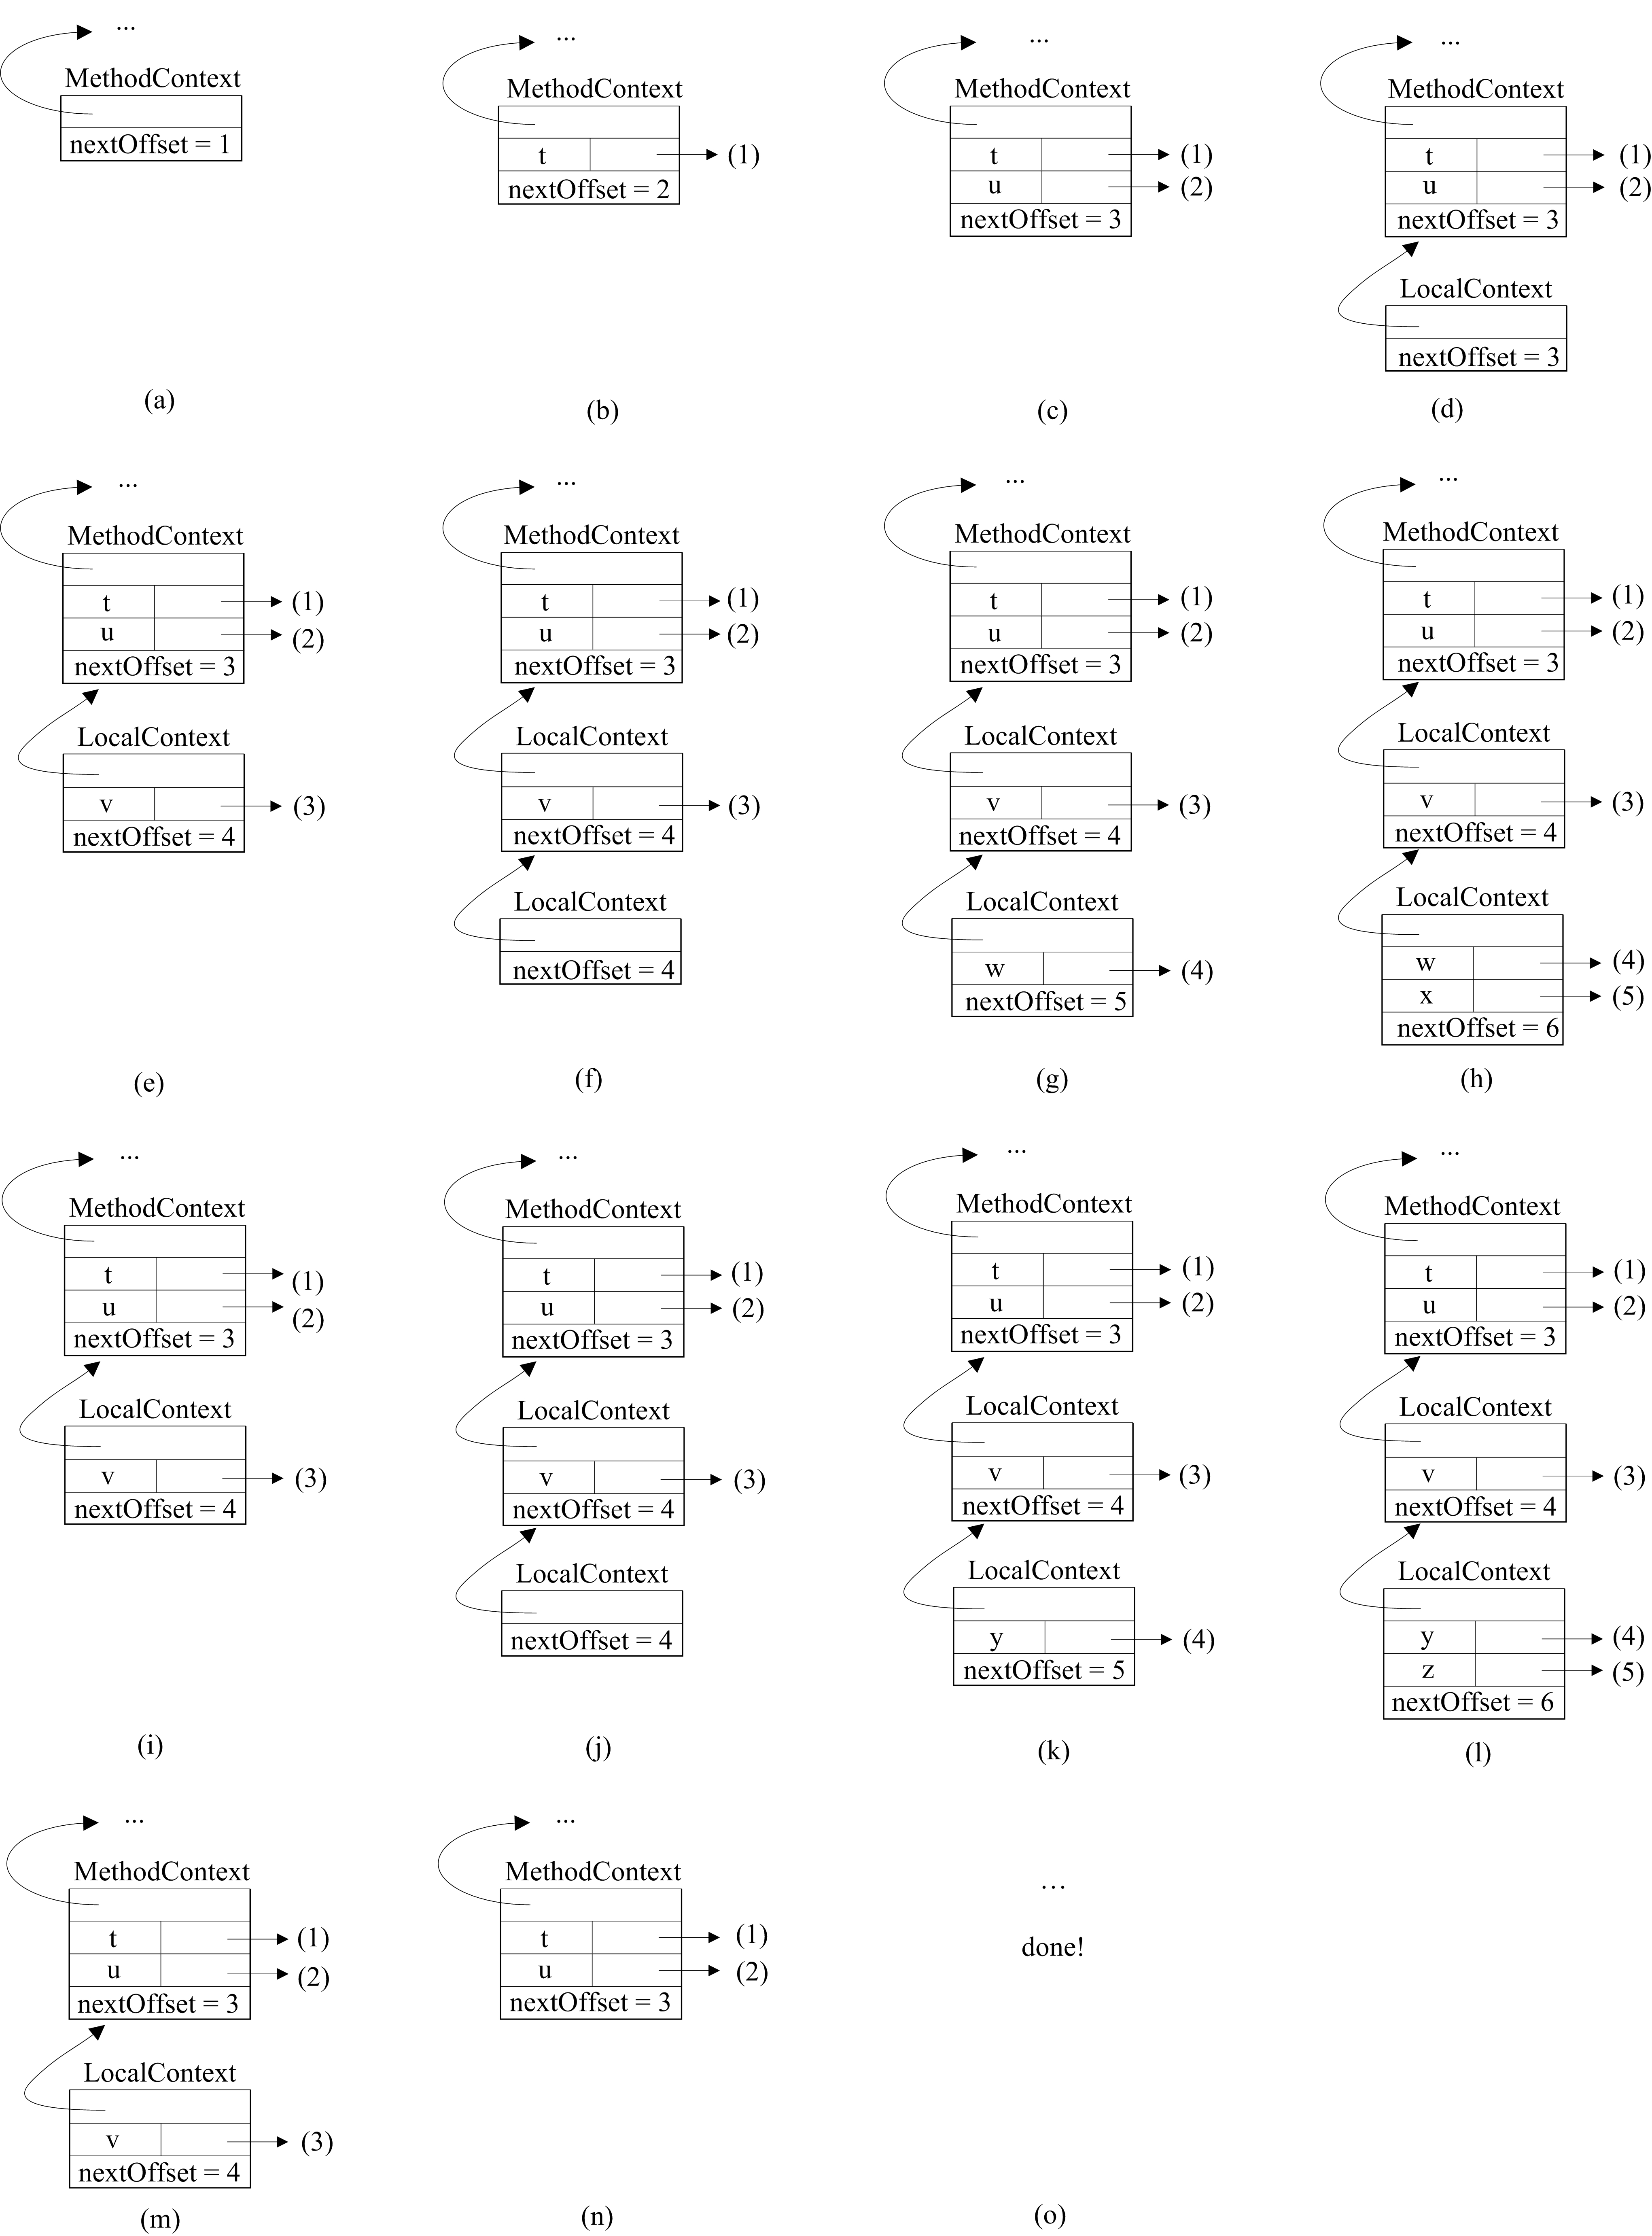
\includegraphics[scale=0.3]{{figures/figure04.07}.jpg}}
\end{center}
\end{frame}

\begin{frame}[fragile]
\pause

A local variable declaration is represented in the AST with a \lstinline{JVariableDeclaration}; for example, consider the local variable declaration from \lstinline{Locals}
\begin{lstlisting}[language=Java,style=focusin]
int w = v + 5, x = w + 7;
\end{lstlisting}

\pause
\bigskip

Before the \lstinline{JVariableDeclaration} is analyzed, it appears exactly as it was created by the parser, as is illustrated below

\begin{center}
\visible<3->{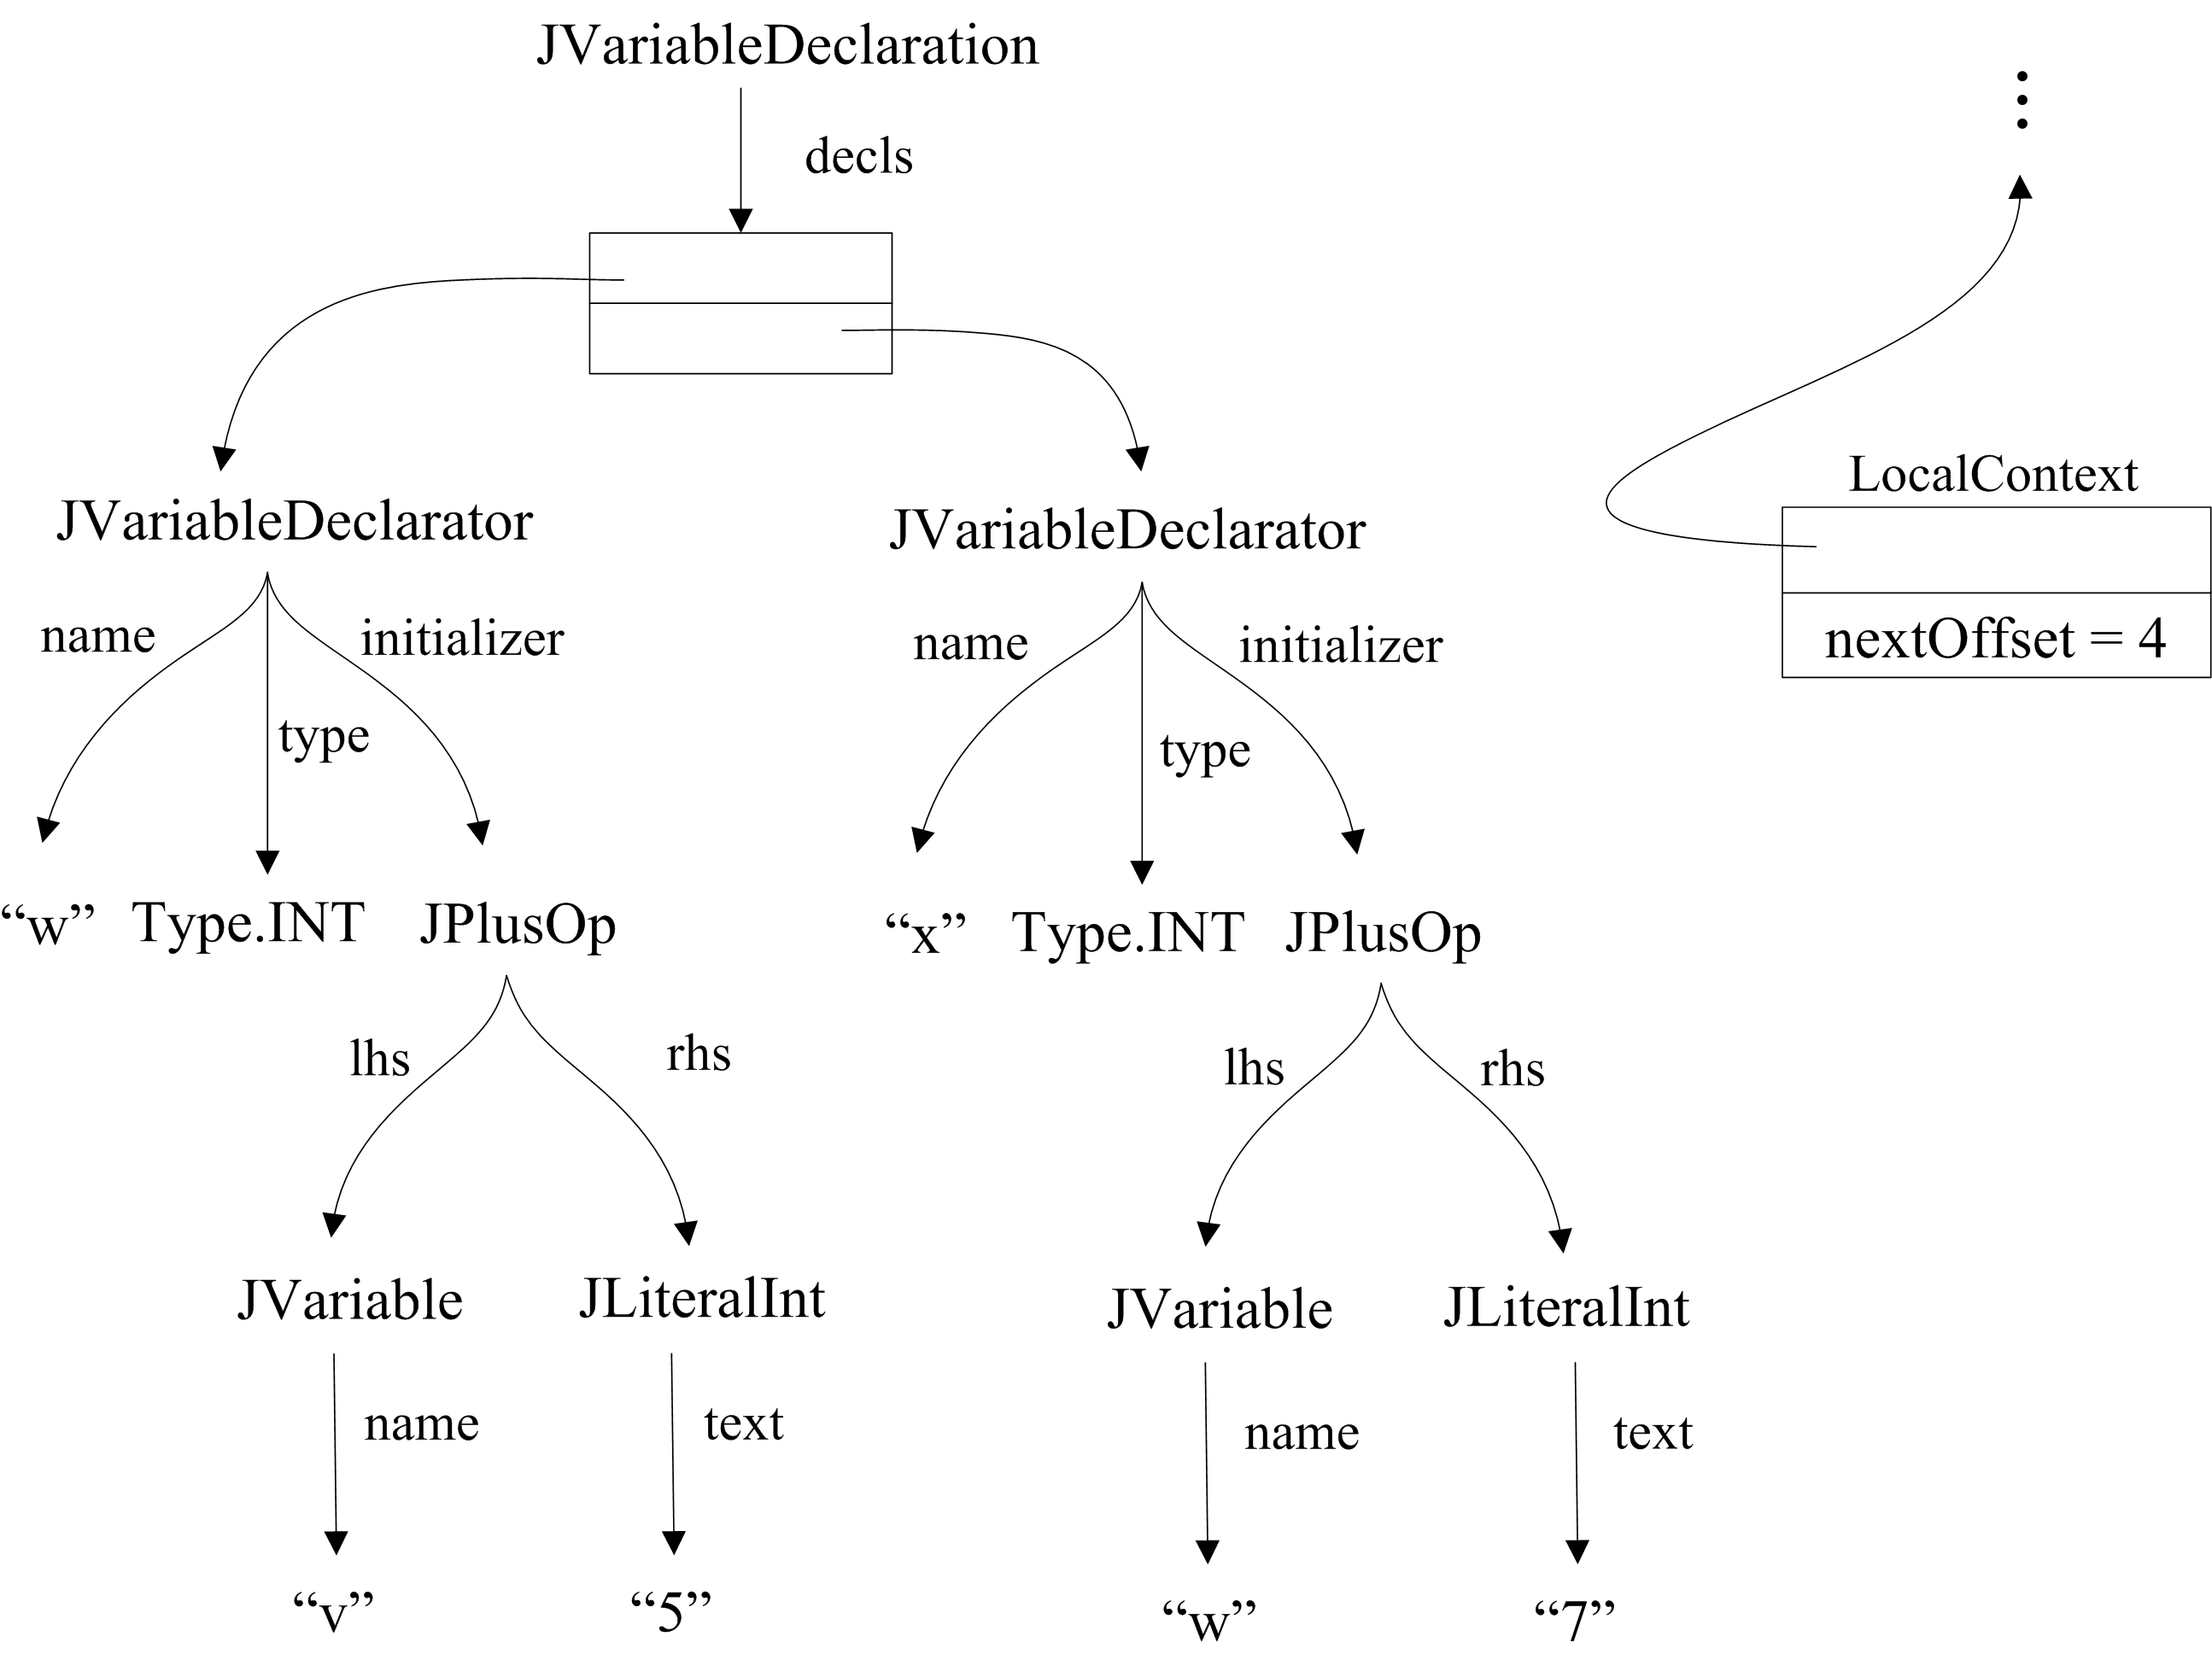
\includegraphics[scale=0.4]{{figures/figure04.08}.jpg}}
\end{center}
\end{frame}

\begin{frame}[fragile]
\pause

Analysis of a \lstinline{JVariableDeclaration} involves the following
\begin{enumerate}
\pause
\item \lstinline{LocalVariableDefn}s and their corresponding stack frame offsets are allocated for each of the declared variables
\pause
\item The code checks to make sure that the declared variables do not shadow existing local variables
\pause
\item The variables are declared in the local context
\pause
\item Any initializations are rewritten as explicit assignment statements; those assignments are re-analyzed and stored in an \lstinline{initializations} list
\end{enumerate}

\pause
\bigskip

\begin{lstlisting}[language=Java,style=focusin]
public JStatement analyze(Context context) {
    for (JVariableDeclarator decl : decls) {
        // Local variables are declared here (fields are
        // declaredin preAnalyze())
        int offset = ((LocalContext) context).nextOffset();
        LocalVariableDefn defn = new LocalVariableDefn(decl
            .type().resolve(context), offset);
\end{lstlisting}
\end{frame}

\begin{frame}[fragile]
\pause

\begin{lstlisting}[language=Java,style=focusin]

        // First, check for shadowing
        IDefn previousDefn = context.lookup(decl.name());
        if (previousDefn != null
            && previousDefn instanceof LocalVariableDefn) {
            JAST.compilationUnit.reportSemanticError(decl.line(),
                "The name " + decl.name()
                    + " overshadows another local variable.");
        }

        // Then declare it in the local context
        context.addEntry(decl.line(), decl.name(), defn);

        // All initializations must be turned into assignment
        // statements and analyzed
        if (decl.initializer() != null) {
             defn.initialize();
            JAssignOp assignOp = new JAssignOp(decl.line(),
                new JVariable(decl.line(), decl.name()), decl
                    .initializer());
            assignOp.isStatementExpression = true;
            initializations.add(new JStatementExpression(decl
                .line(), assignOp).analyze(context));
        }
    }
    return this;
}
\end{lstlisting}
\end{frame}

\begin{frame}[fragile]
\pause

The sub-tree for \lstinline{int w = v + 5, x = w + 7;} after analysis is shown below
\begin{center}
\visible<2->{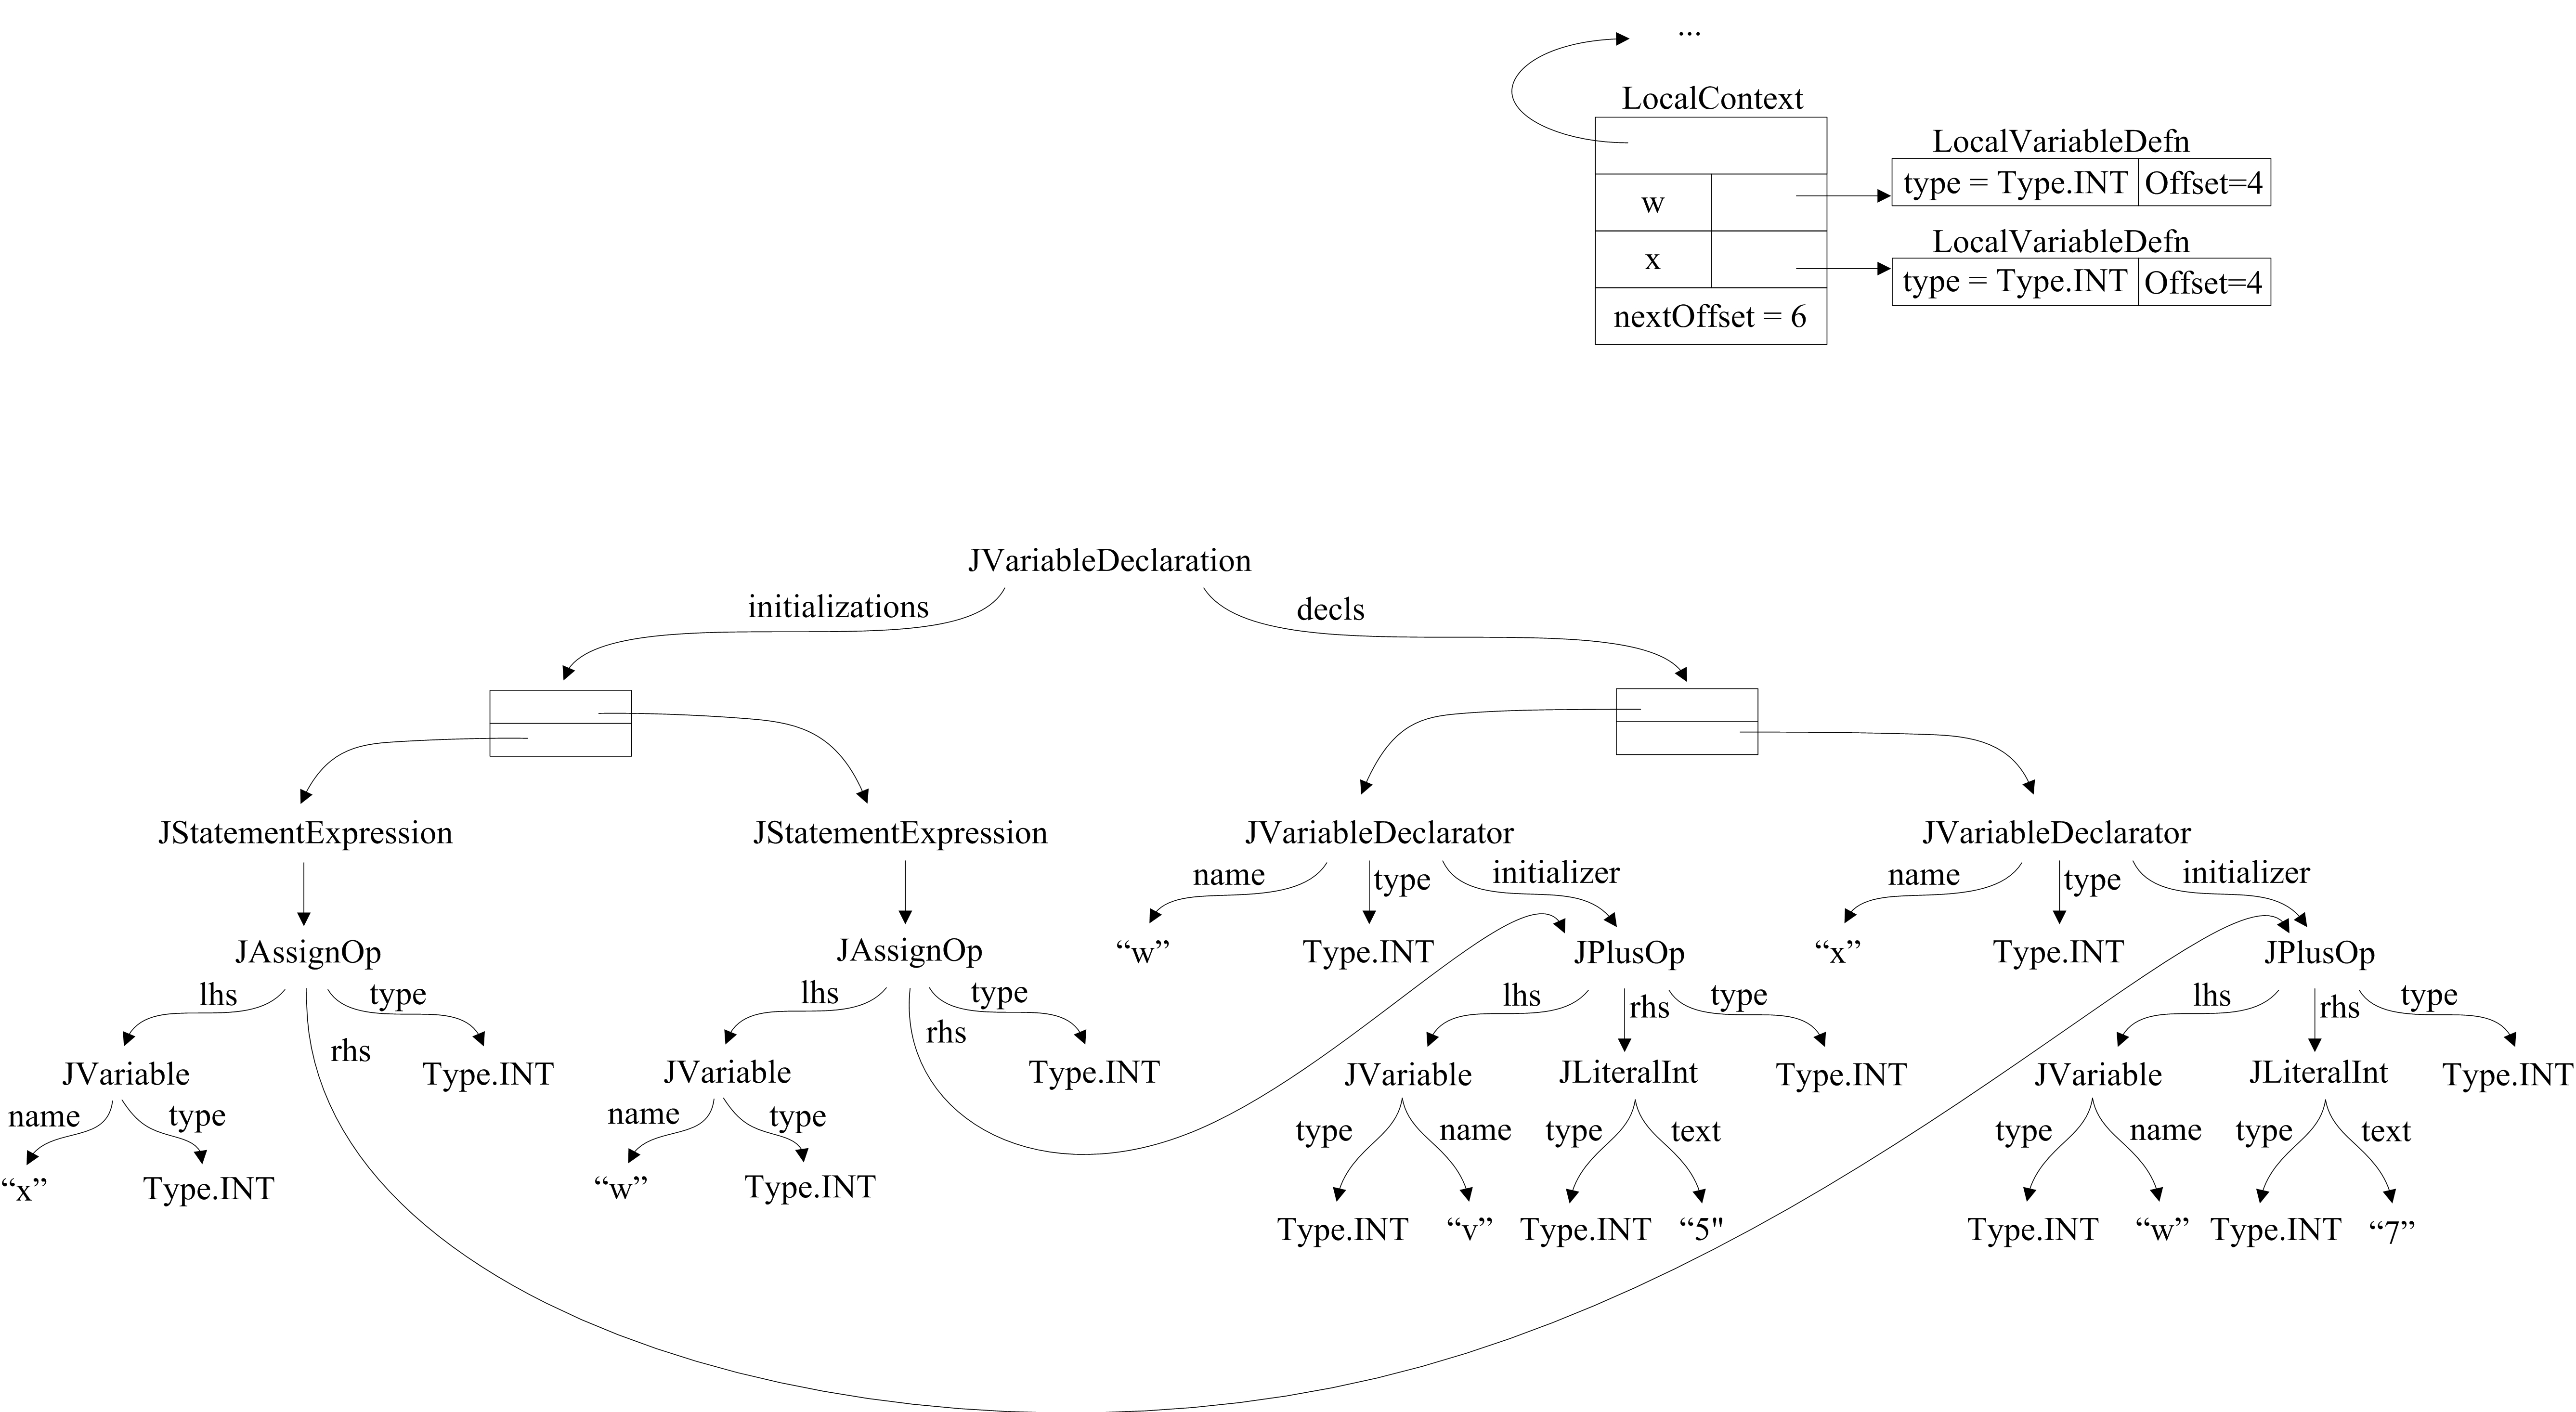
\includegraphics[scale=0.4]{{figures/figure04.09}.jpg}}
\end{center}
\end{frame}

\begin{frame}[fragile]
\pause

Simple variables (local variables or fields) are represented in the AST as \lstinline{JVariable} nodes

\pause
\bigskip

Analysis of simple variables involves looking their names up in the symbol table to find their types

\pause
\bigskip

If a variable is not found in the symbol table, we examine the \lstinline{Type} for the surrounding class (in which the variable appears) to see if it is a field; if it is a field, then the field selection is made explicit by rewriting the tree as a \lstinline{JFieldSelection}

\pause
\bigskip

\begin{lstlisting}[language=Java,style=focusin]
public JExpression analyze(Context context) {
    iDefn = context.lookup(name);
    if (iDefn == null) {
        // Not a local, but is it a field?
	Type definingType = context.definingType();
        Field field = definingType.fieldFor(name);
        if (field == null) {
            type = Type.ANY;
            JAST.compilationUnit.reportSemanticError(line,
                "Cannot find name: " + name);
        } else {
            // Rewrite a variable denoting a field as an
            // explicit field selection
            type = field.type();
            JExpression newTree = new JFieldSelection(line(),
                field.isStatic() ||
		(context.methodContext() != null &&
                 context.methodContext().isStatic()) ?
                        new JVariable(line(),
                            definingType.toString()) :
                            new JThis(line), name);
            return (JExpression) newTree.analyze(context);
        }
\end{lstlisting}
\end{frame}

\begin{frame}[fragile]
\pause

\begin{lstlisting}[language=Java,style=focusin]
    } else {
        if (!analyzeLhs && iDefn instanceof LocalVariableDefn &&
            !((LocalVariableDefn) iDefn).isInitialized()) {
            JAST.compilationUnit.reportSemanticError(line,
                "Variable " + name + " might not have been
                    initialized");
        }
        type = iDefn.type();
    }
    return this;
}
\end{lstlisting}

\pause
\bigskip

For example, the AST node for the local variable \lstinline{v} in the statement \lstinline{return t + v;} in \lstinline{Locals.foo()}, before and after analysis, is shown below
\begin{center}
\visible<3->{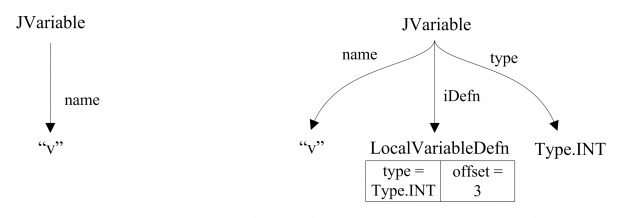
\includegraphics[scale=0.4]{{figures/figure04.10}.jpg}}
\end{center}
\end{frame}

\begin{frame}[fragile]
\pause

As another example, consider the analysis of the static field \lstinline{n}, when it appears in the \lstinline{main()} method of our \lstinline{Factorial} class; the AST node for the field, before and after analysis, is shown below
\begin{center}
\visible<3->{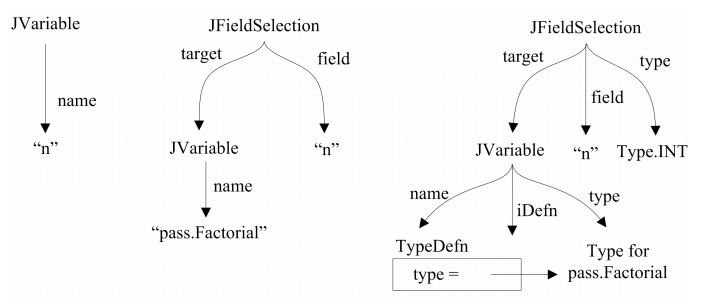
\includegraphics[scale=0.4]{{figures/figure04.11}.jpg}}
\end{center}
\end{frame}

\begin{frame}[fragile]
\pause

Both field selections and message expressions have targets

\pause
\bigskip

In a field selection, the target is either an object or a class from which one wants to select a field, and in a message expression, the target is an object or class to which one is sending a message

\pause
\bigskip

Unfortunately, the parser cannot always make out the syntactic structure of a target

\pause
\bigskip

For example, consider the field selection \lstinline{w.x.y.z}; the parser knows this is a field selection of some sort and that \lstinline{z} is the field, but, without knowing the types of \lstinline{w}, \lstinline{x} and \lstinline{y}, the parser cannot know whether
\begin{itemize}
\pause
\item \lstinline{w} is a class name,  \lstinline{x} is a static field in \lstinline{w}, and \lstinline{y} is a field of \lstinline{x};
\pause
\item \lstinline{w} is a package containing class \lstinline{x}, and \lstinline{y} is a static field in \lstinline{x}; or
\pause
\item \lstinline{w.x.y} is a fully qualified class name like \lstinline{java.lang.System}
\end{itemize}

\pause
\bigskip

For this reason, the parser packages up the string \lstinline{"w.x.y"} in an \lstinline{AmbiguousName} object, attached to either the \lstinline{JFieldSelection} or \lstinline{JMessageExpression}, deferring the decision until analysis

\pause
\bigskip

The \lstinline{reclassify()} method in \lstinline{AmbiguousName} is based on the rules in the Java Language Specification for reclassifying an ambiguous name
\end{frame}

\begin{frame}[fragile]
\pause

\begin{lstlisting}[language=Java,style=focusin]
public JExpression reclassify(Context context) {
    // Easier because we require all types to be imported.
    JExpression result = null;
    StringTokenizer st = new StringTokenizer(name, ".");

    // Firstly, find a variable or Type.
    String newName = st.nextToken();
    IDefn iDefn = null;

    do {
        iDefn = context.lookup(newName);
        if (iDefn != null) {
            result = new JVariable(line, newName);
            break;
        } else if (!st.hasMoreTokens()) {
            // Nothing found. :(
            JAST.compilationUnit.reportSemanticError(line,
                "Cannot find name " + newName);
            return null;
        } else {
            newName += "." + st.nextToken();
        }
    } while (true);

    // For now we can assume everything else is fields.
    while (st.hasMoreTokens()) {
        result = new JFieldSelection(line, result, st.nextToken());
    }
    return result;
}
\end{lstlisting}
\end{frame}

\begin{frame}[fragile]
\pause

For example, consider the message expression
\begin{lstlisting}[language=Java,style=focusin]
java.lang.System.out.println(...);
\end{lstlisting}

The parser will have encapsulated the target \lstinline{java.lang.System.out} in an \lstinline{AmbiguousName} object

\pause
\bigskip

The first thing \lstinline{analyze()} does for a \lstinline{JMessageExpression} is to reclassify the \lstinline{AmbiguousName} to determine the structure of the expression that it denotes, which it does by looking at the ambiguous \lstinline{java.lang.System.out} from left to right
\begin{enumerate}
\pause
\item Firstly, \lstinline{reclassify(}) looks up the simple name, \lstinline{java} in the symbol table.
\pause
\item Not finding that, it looks up \lstinline{java.lang}
\pause
\item Not finding that, it looks up \lstinline{java.lang.System}, which (assuming \lstinline{java.lang.System} has been properly imported) it finds to be a class.
\pause
\item It then assumes that the rest of the ambiguous part, that is \lstinline{out}, is a field
\pause
\item Thus the target is a field selection whose target is \lstinline{java.lang.System} and whose field name is \lstinline{out}
\end{enumerate}
\end{frame}

\begin{frame}[fragile]
\pause

After reclassifying any ambiguous part and making that the target, analysis of a \lstinline{JFieldSelection} proceeds as follows
\begin{enumerate}
\pause
\item It analyzes the target and determines the target's type
\pause
\item It then considers the special case where the target is an array and the field is \lstinline{length}.  In this case, the type of the ``field selection'' is \lstinline{Type.INT}
\pause
\item Otherwise, it ensures that the target is not a primitive and determines whether or not it can find a field of the appropriate name in the target's type; if it cannot, then an error is reported
\pause
\item Otherwise, it checks to make sure the field is accessible to this region, a non-static field is not referenced from a static context, and then returns the analyzed field selection sub-tree
\end{enumerate}

\pause
\bigskip

\begin{lstlisting}[language=Java,style=focusin]
public JExpression analyze(Context context) {
    // Reclassify the ambiguous part.
    ...
    
    target = (JExpression) target.analyze(context);
    Type targetType = target.type();
    
    // We use a workaround for the "length" field of arrays.
    if ((targetType instanceof ArrayTypeName) && fieldName.equals("length")) {
        type = Type.INT;
    } else {
        // Other than that, targetType has to be a
        // ReferenceType
        if (targetType.isPrimitive()) {
            JAST.compilationUnit.reportSemanticError(line(),
                "Target of a field selection must be a defined type");
            type = Type.ANY;
            return this;
        }
\end{lstlisting}
\end{frame}

\begin{frame}[fragile]
\pause

\begin{lstlisting}[language=Java,style=focusin]
        field = targetType.fieldFor(fieldName);
        if (field == null) {
            JAST.compilationUnit.reportSemanticError(line(),
                "Cannot find a field: " + fieldName);
            type = Type.ANY;
        } else {
            context.definingType().checkAccess(line,
		(Member) field);
            type = field.type();

            // Non-static field cannot be referenced from a
            // static context.
            if (!field.isStatic()) {
                if (target instanceof JVariable &&
                    ((JVariable) target).iDefn() instanceof
                       TypeNameDefn) {
                     JAST.compilationUnit.
                         reportSemanticError(line(),
                         "Non-static field " + fieldName +
                            " cannot be referenced from a static
                              context");
                }
            }
        }
    }
    return this;
}
\end{lstlisting}
\end{frame}

\begin{frame}[fragile]
\pause

After reclassifying any \lstinline{AmbiguousName}, analyzing a \lstinline{JMessageExpression} proceeds as follows

\begin{enumerate}
\pause
\item It analyzes the arguments to the message and constructs an array of their types
\pause
\item It determines the surrounding, defining class (for determining access)
\pause
\item It analyzes the target to which the message is being sent
\pause
\item It takes the message name and the array of argument types and looks for a matching method defined in the target's type (in \jmm, argument types must match exactly), and if no such method is found, it reports an error
\pause
\item Otherwise, the target class and method are checked for accessibility, a non-static method is now allowed to be referenced from a static context, and the method's return type becomes the type of the message expression
\end{enumerate}

\begin{lstlisting}[language=Java,style=focusin]
public JExpression analyze(Context context) {
    // Reclassify the ambiguous part
    …

    // Then analyze the arguments, collecting
    // their types (in Class form) as argTypes
    argTypes = new Type[arguments.size()];
    for (int i = 0; i < arguments.size(); i++) {
        arguments.set(i, (JExpression) arguments.get(i).analyze(
            context));
        argTypes[i] = arguments.get(i).type();
    }
\end{lstlisting}
\end{frame}

\begin{frame}[fragile]
\pause

\begin{lstlisting}[language=Java,style=focusin]

    // Where are we now? (For access)
    Type thisType = ((JTypeDecl) context.classContext
        .definition()).thisType();
        
    // Then analyze the target
    if (target == null) {
                 // Implied this (or, implied type for statics)
        if (!context.methodContext().isStatic()) {
            target = new JThis(line()).analyze(context);
        }
        else {
            target = new JVariable(line(),
                        context.definingType().toString()).
                            analyze(context);
        }
    } else {
        target = (JExpression) target.analyze(context);
        if (target.type().isPrimitive()) {
            JAST.compilationUnit.reportSemanticError(line(),
                "cannot invoke a message on a primitive type:"
                    + target.type());
        }
    }
\end{lstlisting}
\end{frame}

\begin{frame}[fragile]
\pause

\begin{lstlisting}[language=Java,style=focusin]

    // Find appropriate Method for this message expression
    method = target.type().methodFor(messageName, argTypes);
    if (method == null) {
        JAST.compilationUnit.reportSemanticError(line(),
            "Cannot find method for: "
                + Type.signatureFor(messageName, argTypes));
        type = Type.ANY;
    } else {
        context.definingType().checkAccess(line,
                                          (Member) method);
        type = method.returnType();

        // Non-static method cannot be referenced from a
        // static context.
        if (!method.isStatic()) {
            if (target instanceof JVariable &&
                ((JVariable) target).iDefn() instanceof
                    TypeNameDefn) {
                 JAST.compilationUnit.reportSemanticError(line(),
                  "Non-static method " +
                  Type.signatureFor(messageName, argTypes) +
                  "cannot be referenced from a static context");
            }
        }
    }
    return this;
}
\end{lstlisting}
\end{frame}

\begin{frame}[fragile]
\pause

The rest of analysis, as defined for the various kinds of AST nodes is about computing and checking types and enforcing additional \jmm rules

\pause
\bigskip

For most kinds of AST nodes, analysis involves analyzing the sub-trees and checking the types

\pause
\bigskip

Analysis of \lstinline{JIfStatement}
\begin{lstlisting}[language=Java,style=focusin]
public JStatement analyze(Context context) {
    test = (JExpression) test.analyze(context);
    test.type().mustMatchExpected(line(), Type.BOOLEAN);
    consequent = (JStatement) consequent.analyze(context);
    if (alternate != null) {
        alternate = (JStatement) alternate.analyze(context);
    }
    return this;
}
\end{lstlisting}

\pause
\bigskip

Analysis of \lstinline{JSubtractOp}
\begin{lstlisting}[language=Java,style=focusin]
public JExpression analyze(Context context) {
     lhs = (JExpression) lhs.analyze(context);
     rhs = (JExpression) rhs.analyze(context);
     lhs.type().mustMatchExpected(line(), Type.INT);
     rhs.type().mustMatchExpected(line(), Type.INT);
     type = Type.INT;
     return this;
 }
\end{lstlisting}
\end{frame}

\begin{frame}[fragile]
\pause

Analysis of \lstinline{JPlusOp}
\begin{lstlisting}[language=Java,style=focusin]
public JExpression analyze(Context context) {
    lhs = (JExpression) lhs.analyze(context);
    rhs = (JExpression) rhs.analyze(context);
    if (lhs.type() == Type.STRING || rhs.type() == Type.STRING) {
        return (new JStringConcatenationOp(line, lhs, rhs))
            .analyze(context);
    } else if (lhs.type() == Type.INT && rhs.type() == Type.INT){
        type = Type.INT;
    } else {
        type = Type.ANY;
        JAST.compilationUnit.reportSemanticError(line(),
            "Invalid operand types for +");
    }
    return this;
}
\end{lstlisting}

\pause
\bigskip

Analysis of \lstinline{JStringConcatenateOp}
\begin{lstlisting}[language=Java,style=focusin]
public JExpression analyze(Context context) {
    type = Type.STRING;
    return this;
}
\end{lstlisting}

\pause
\bigskip

Analysis of \lstinline{JLiteralInt}
\begin{lstlisting}[language=Java,style=focusin]
public JExpression analyze(Context context) {
    type = Type.INT;
    return this;
}
\end{lstlisting}
\end{frame}

\begin{frame}[fragile]
\pause

The \jmm language is stricter than is Java when it comes to types

\pause
\bigskip

There are no implied conversions in \jmm; when one assigns an expression to a variable, the types must match exactly, and the same goes for actual parameters to messages matching the formal parameters of methods

\pause
\bigskip

This does not exclude polymorphism; for example if type \lstinline{Bar} extends type \lstinline{Foo}, if \lstinline{bar} is a variable of type \lstinline{Bar} and \lstinline{foo} is a variable of type \lstinline{Foo}, we can say
\begin{lstlisting}[language=Java,style=focusin]
foo = (Foo) bar;
\end{lstlisting}
to keep the \jmm compiler happy

\pause
\bigskip

Of course, the object that \lstinline{bar} refers to could be of type \lstinline{Bar} or any of its sub-types; polymorphism has not gone away

\pause
\bigskip

Analysis, when encountering a \lstinline{JCastOp}\index{\lstinline{JCastOp}} for an expression such as 
\begin{lstlisting}[language={},style=focusin]
    (Type2) expression of Type1
\end{lstlisting}
must determine two things
\begin{enumerate}
\pause
\item That an expression of type \lstinline{Type1} can be cast to \lstinline{Type2}, ie, that the cast is valid
\pause
\item The type of the result, which is simply \lstinline{Type2}
\end{enumerate}
\end{frame}

\begin{frame}[fragile]
\pause

To determine (1) we must consider the possibilities for \lstinline{Type1} and \lstinline{Type2}
\begin{enumerate}
\pause
\item Any type may be cast to itself (aka identity cast)
\pause
\item An arbitrary reference type may be cast to another reference type if and only if either one of the following holds
\begin{enumerate}
\pause
\item The first type is a sub-type of (extends) the second type; this is called widening and requires no action at run time
\pause
\item The second type is a sub-type of the first type; this is called narrowing and requires a run-time check to make sure the expression being cast is actually an instance of the type it is being cast to
\end{enumerate}
\pause
\item The following table summarizes other casts, and says whether or not (and how) a type labeling a row may be cast to a type labeling a column
\begin{center}
    \begin{tabular}{ | l | l | l | l | l | l | l | }
    \hline
    & \lstinline$boolean$   & \lstinline$char$    & \lstinline$int$ & \lstinline$Boolean$ &
                \lstinline$Character$ & \lstinline$Integer$   \\ \hline

   \lstinline$boolean$   & Identity & Error     & Error    & Boxing  & Error  & Error \\ \hline
   \lstinline$char$      & Error    & Identity  & Widening & Error   & Boxing & Error \\ \hline
   \lstinline$int$       & Error    & Narrowing & Identity & Error   & Error      & Boxing \\ \hline
   \lstinline$Boolean$   & Unboxing & Error     & Error    & Identity & Error   & Error \\ \hline
   \lstinline$Character$ & Error    & Unboxing  & Error    & Error    & Identity & Error \\ \hline
   \lstinline$Integer$   & Error    & Error     & Unboxing & Error    & Error   & Identity \\ \hline
    \end{tabular}
\end{center}
\end{enumerate}
\end{frame}

\begin{frame}[fragile]
\pause

Analysis in \lstinline{JCastOp}

\begin{lstlisting}[language=Java,style=focusin]
public JExpression analyze(Context context) {
    expr = (JExpression) expr.analyze(context);
    type = cast = cast.resolve(context);
    if (cast.equals(expr.type())) {
        converter = Converter.Identity;
    } else if (cast.isJavaAssignableFrom(expr.type())) {
        converter = Converter.WidenReference;
    } else if (expr.type().isJavaAssignableFrom(cast)) {
        converter = new NarrowReference(cast);
    } else if ((converter =
        conversions.get(expr.type(), cast)) != null) {
    } else {
        JAST.compilationUnit.reportSemanticError(line,
            "Cannot cast a " + expr.type().toString() + " to a "
                + cast.toString());
    }
    return this;
}
\end{lstlisting}

\pause
\bigskip

A converter for narrowing one reference type to another (more specific) reference sub-type
\begin{lstlisting}[language=Java,style=focusin]
class NarrowReference implements Converter {
    private Type target;

    public NarrowReference(Type target) {
        this.target = target;
    }

    public void codegen(CLEmitter output) {
        output.addReferenceInstruction(CHECKCAST, target.jvmName());
    }
}
\end{lstlisting}
\end{frame}

\begin{frame}[fragile]
\pause

In Java, every variable (whether it be a local variable or a field) must be definitely assigned before it is accessed in a computation, ie, it must appear on the left hand side of the \lstinline{=} operator before it is accessed

\pause
\bigskip

We do not have this rule in  \jmm, so we need not enforce it in our compiler

\pause
\bigskip

Enforcing the definite assignment rule requires data flow analysis, which determines where in the program variables are defined (assigned values), where in the program the variables' values are used and so where in the program those values are valid (from assignment to last use)

\pause
\bigskip

Our JVM to MIPS translator performs data-flow analysis as part of computing live intervals for register allocation
\end{frame}
\end{document}
